\documentclass{report}

\usepackage[T1]{fontenc}
\usepackage{geometry}
\usepackage{graphicx}
\usepackage{multicol}
\usepackage{pgffor}
\usepackage{tikz}
\usepackage{caption}
\usepackage{amsmath}
\geometry{
    a4paper,
    total={170mm,257mm},
    left=5mm,
    right=10mm,
    top=20mm,
}

\title{Matt study, Nuclear transparency}
\date{2024\\ September}
\author{Mathieu Ouillon}

\begin{document}
\maketitle

\section{Strategy}
\subsection{Carbon target}
    Carbon runs : 018339, 018340, 018341, 018342, 018343, 018344, 018346, 018440, 018441, 018442, 018443, 018444, 018445, 018475, 018498, 018524, 018756, 018850
    
    path: \texttt{/cache/hallb/scratch/rg-d/production/Bspot/v5dstCxC/dst/recon/}
    \begin{itemize}
        \item Find event with a trigger electron(\texttt{REC::Particle::pid == 11} and \texttt{status<0}), at least a \(\pi^+\) and at least a \(\pi^-\).
        \item Apply cut on electron: \(-5 < \chi^2_{pid} < 5\) and \(-12 < v_z < 5\)
        \item Find all \(\pi^+\) in event: \texttt{REC::Particle::pid == 211}
        \item Apply cut on \(\pi^+\): \(-10 < \chi^2_{pid} < 10\) 
        \item Find all \(\pi^-\) in event: \texttt{REC::Particle::pid == -211}
        \item Apply cut on \(\pi^-\): \(-10 < \chi^2_{pid} < 10\)
        \item Find all combinaison of \(\pi^+\) and \(\pi^-\)
        \item Cut to select reaction : 
        \begin{itemize}
            \item \(W = (p_i + \gamma^{\star})^2 > 2GeV\), with \(p_i = (0,0,0,M_p)\), \(M_p = 0.938 GeV^2\)
            \item \(z_h = \frac{E_{\rho^0}}{v}> 0.9\)
            \item \( 0.1 < -t = (\gamma^{\star} - p_{\rho^0})^2 < 0.5 GeV^2\)
            \item \(l_c \le 0.5 fm\)
        \end{itemize}
        \item Fill invariant mass of \(\rho^0\) for the \(Q^2\) bins : \(1 \le Q^2 < 2\), \(2 \le Q^2 < 2.5\), \(2.5 \le Q^2 < 3\), \(3 \le Q^2 < 3.5\), \(3.5 \le Q^2 < 4.5\), \(4.5 \le Q^2 < 6\)
        \item Fit the distribution with a Breit-Wigner and a 3rd order polynom between 0.3 and 1.4 \(GeV/c^2\): 
        \begin{align}
            \text{BW}(x;x_0,\Gamma,\alpha) = \alpha \times \frac{1}{\pi} \times \frac{\frac{1}{2}\Gamma}{(x-x_0)^2 + \frac{1}{2}\Gamma} \\
            \text{pol3}(x;a,b,c,d) = a + b \times x + c \times x^2 + d \times x^3
        \end{align}
        where \(x_{0}\) is the location parameter, specifying the location of the peak of the distribution, \(\gamma\) is full width at half maximum (FWHM).
        \item Take the integral of the fit function using \texttt{Integral} root function between 0.3 and 1.4 \(GeV/c^2\).
    \end{itemize}

    \section{Carbon data}
    \subsection{Numbers}
    
    \begin{itemize}
        \item Total number of event : 354888652
        \item Number of event with a trigger electron (\texttt{REC::Particle::pid == 11} and \texttt{status<0}) and at least a \(\pi^+\) and at least a \(\pi^-\) : 22585713; ratio between this one and the previous number : 0.0636417
        \item Number of event with a good electron : 20067249; ratio : 0.888493
        \item Number of \(\pi^+\) after electron cuts: 27575088
        \item Number of good \(\pi^+\) after electron and \(\pi^+\) cuts : 18219354; ratio : 0.660718
        \item Number of bad \(\pi^+\) after electron and opposite \(\pi^+\) cuts: 9355734; ratio : 0.339282
        \item Number of \(\pi^-\) after electron cuts: 25090248
        \item Number of good \(\pi^-\) after electron and \(\pi^-\) cuts: 20446619; ratio : 0.814923
        \item Number of bad \(\pi^-\) after electron and opposite \(\pi^-\) cuts: 4643629; ratio : 0.185077
        \item Number of \(\rho^0\) : 20411533;
        \item Number of \(\rho^0\) that pass the \(W\) cut : 19735078; ratio : 0.966859
        \item Number of \(\rho^0\) that pass the \(W\) and \(z_h\) cuts : 355804; ratio : 0.018029
        \item Number of \(\rho^0\) that pass the \(W\), \(z_h\) and \(t\) cuts : 163572; ratio : 0.459725
        \item Number of \(\rho^0\) that pass the \(W\), \(z_h\), \(t\) and \(l_c\) cuts : 10173; ratio : 0.0621928
    \end{itemize}
    

    

    

    

    \subsection{Electron}
    \begin{minipage}{.5\textwidth}
        \centering
        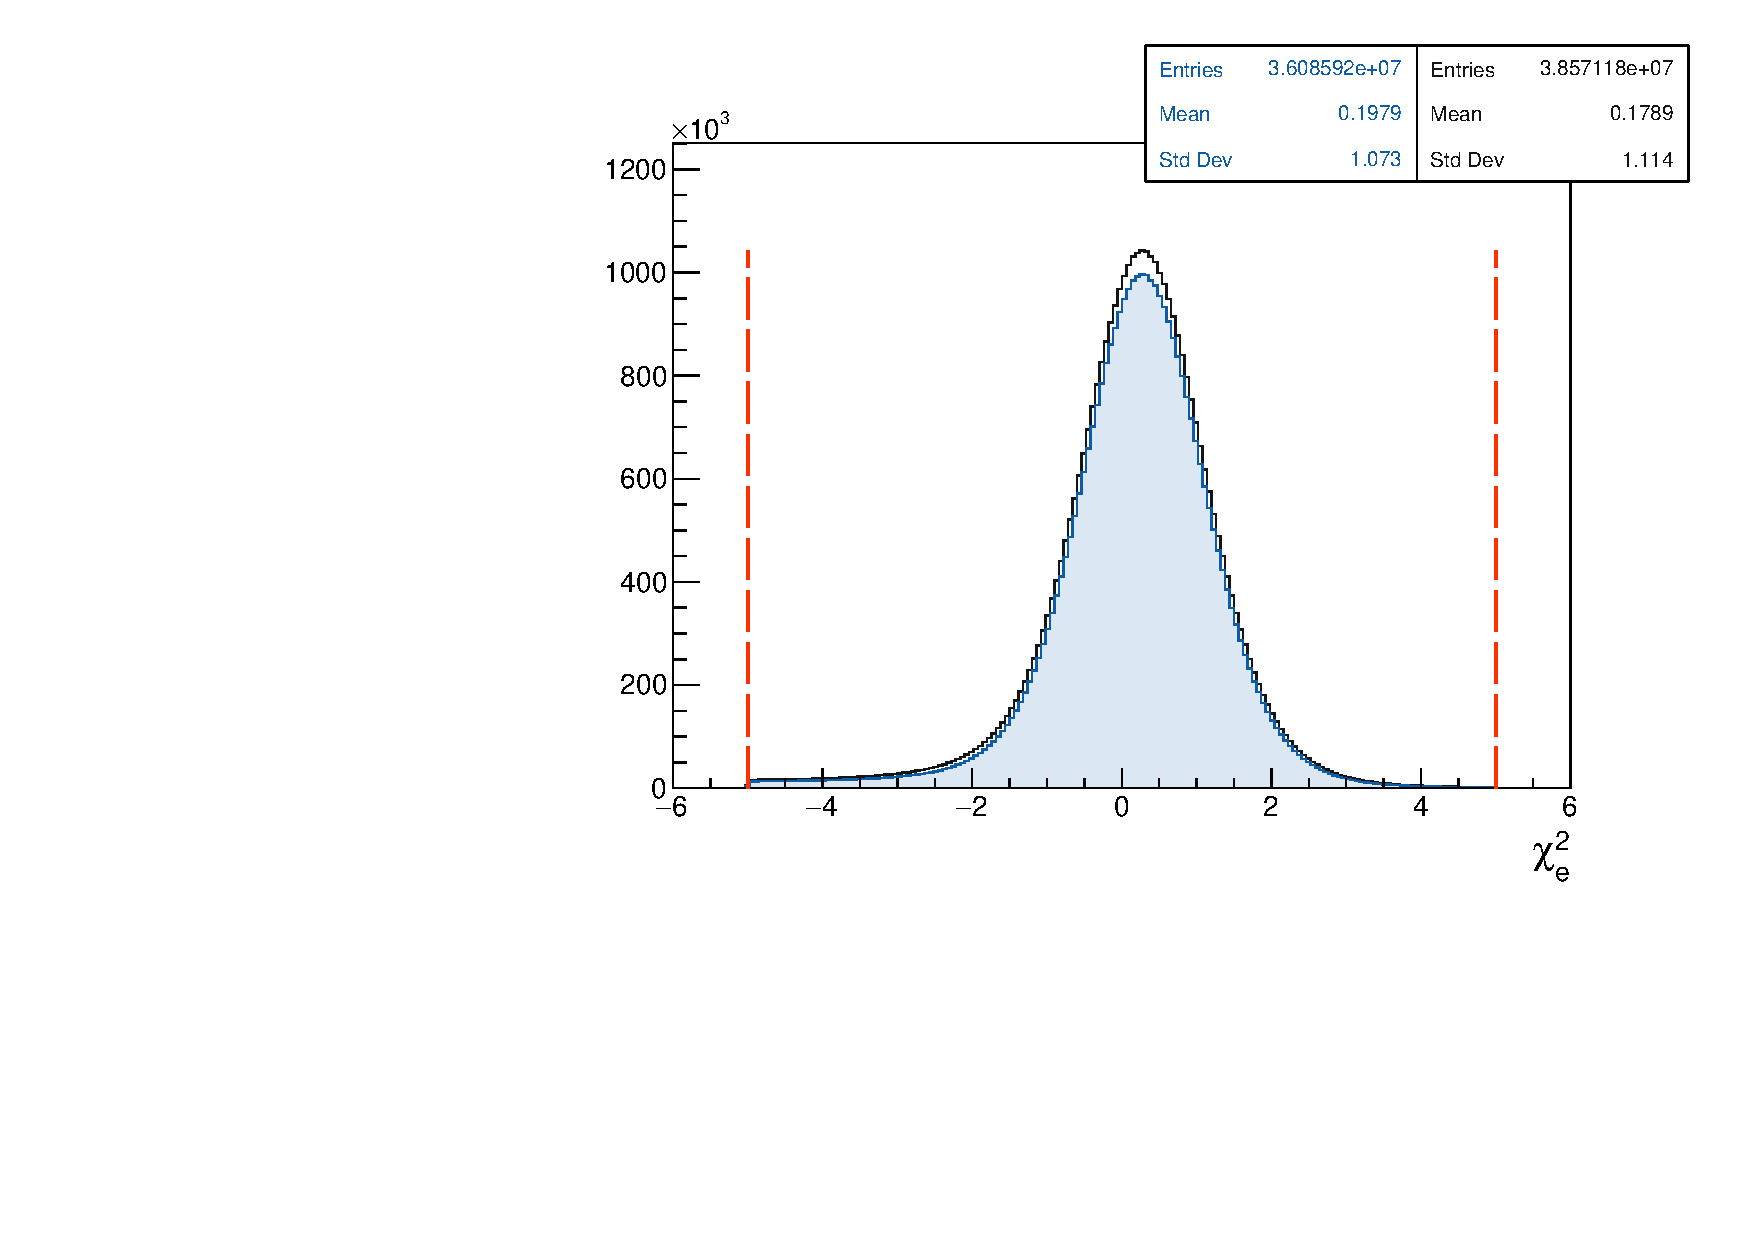
\includegraphics[width=280pt]{/work/clas12/ouillon/Analysis_RG-D/plots_Matt_Study/CxC/electron_kinematics/pdf/chi2_e.pdf}
    \end{minipage}
    \begin{minipage}{.5\textwidth}
        \centering
        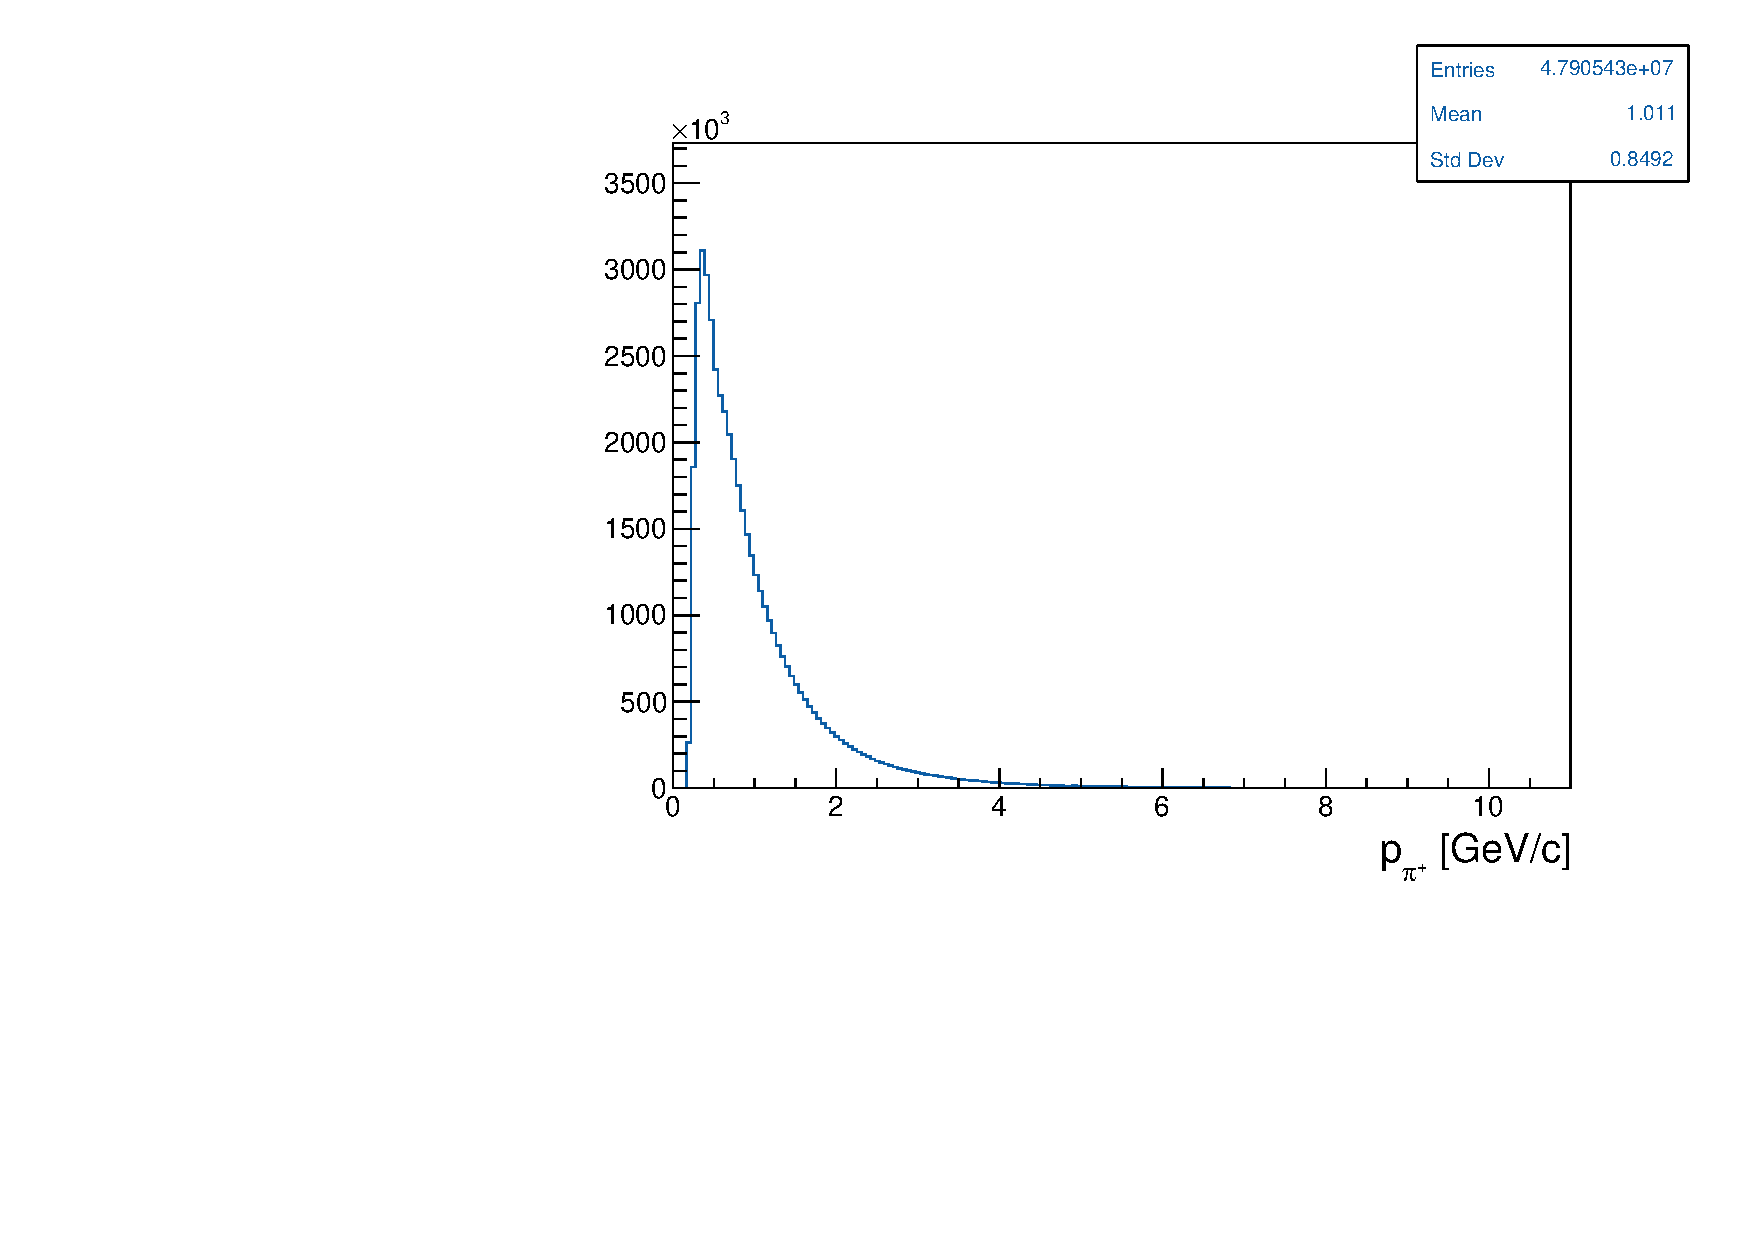
\includegraphics[width=280pt]{/work/clas12/ouillon/Analysis_RG-D/plots_Matt_Study/CxC/electron_kinematics/pdf/p_e.pdf}
    \end{minipage}

    \begin{minipage}{.5\textwidth}
        \centering
        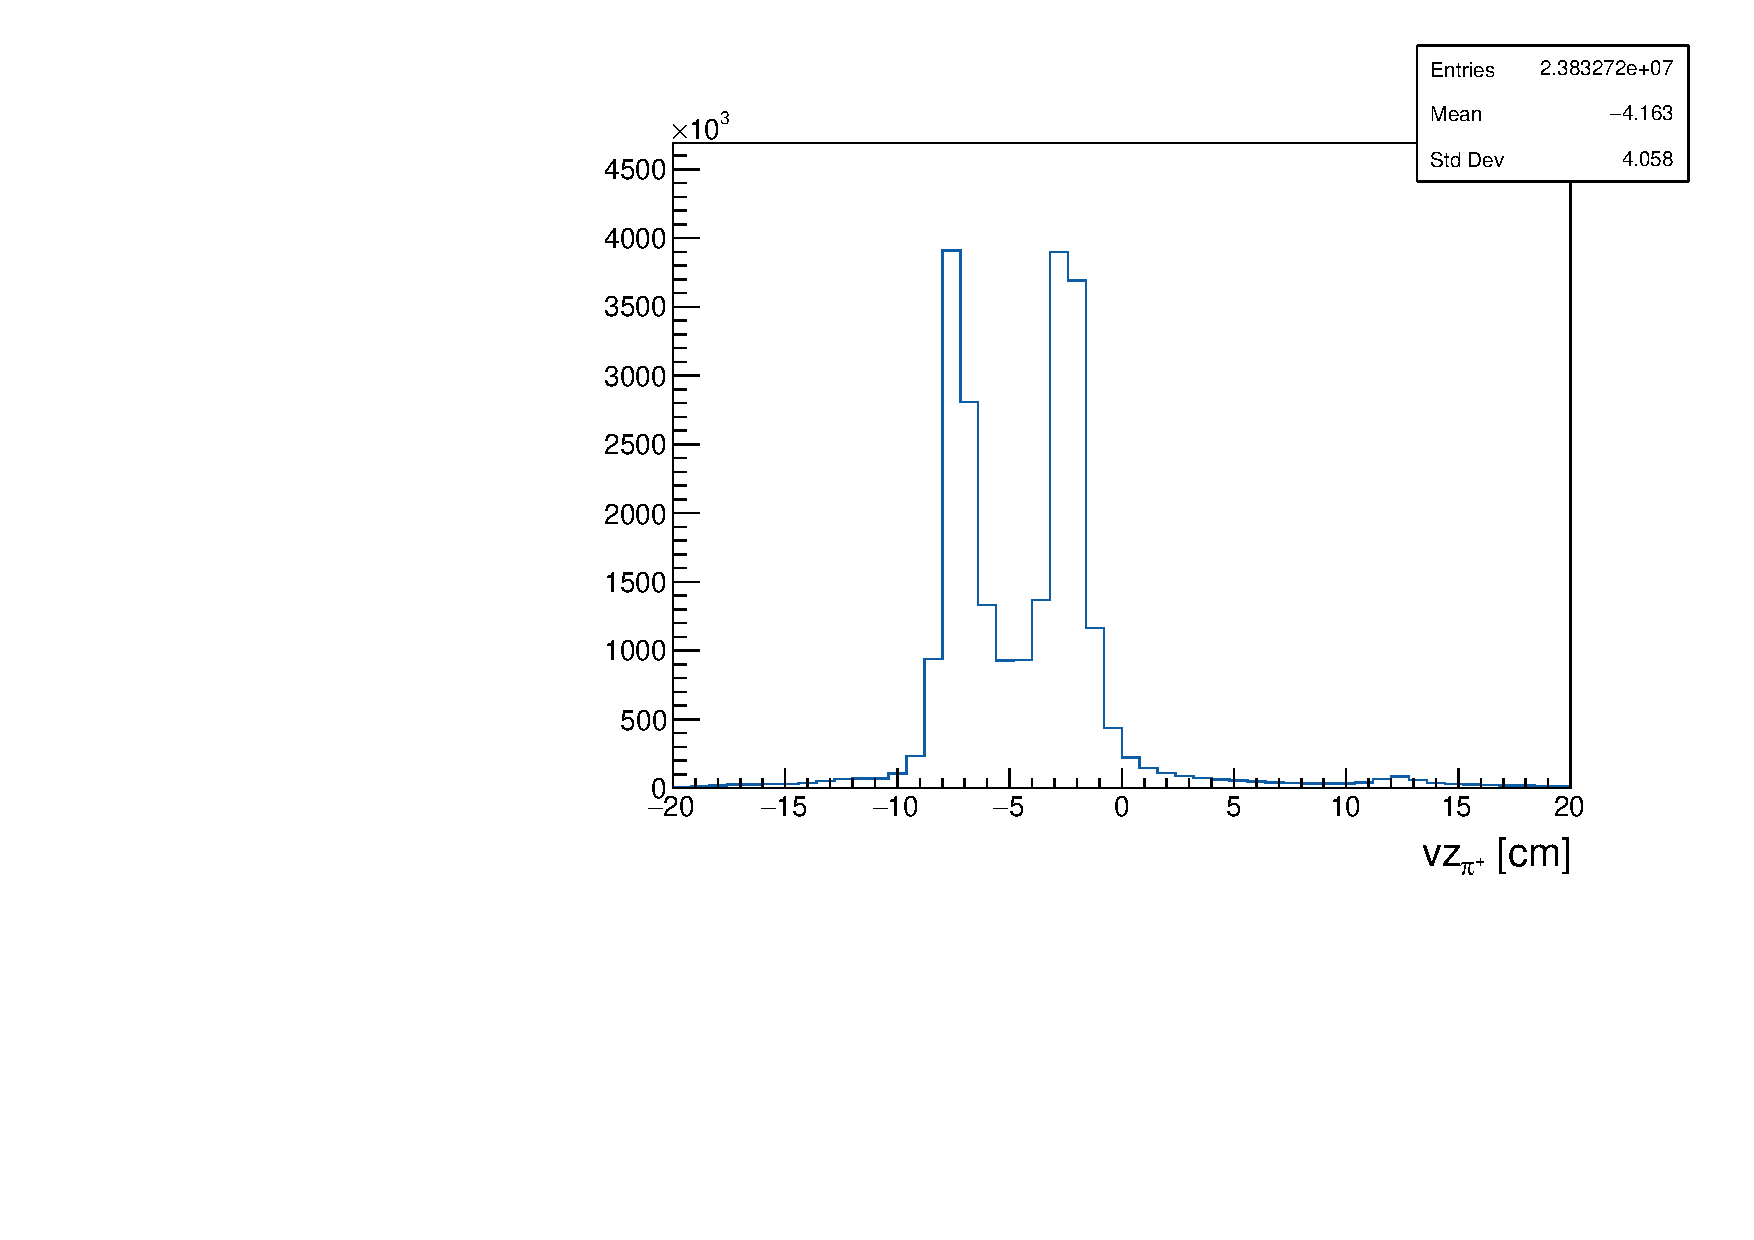
\includegraphics[width=280pt]{/work/clas12/ouillon/Analysis_RG-D/plots_Matt_Study/CxC/electron_kinematics/pdf/vz_e.pdf}
    \end{minipage}
    \begin{minipage}{.5\textwidth}
        \centering
        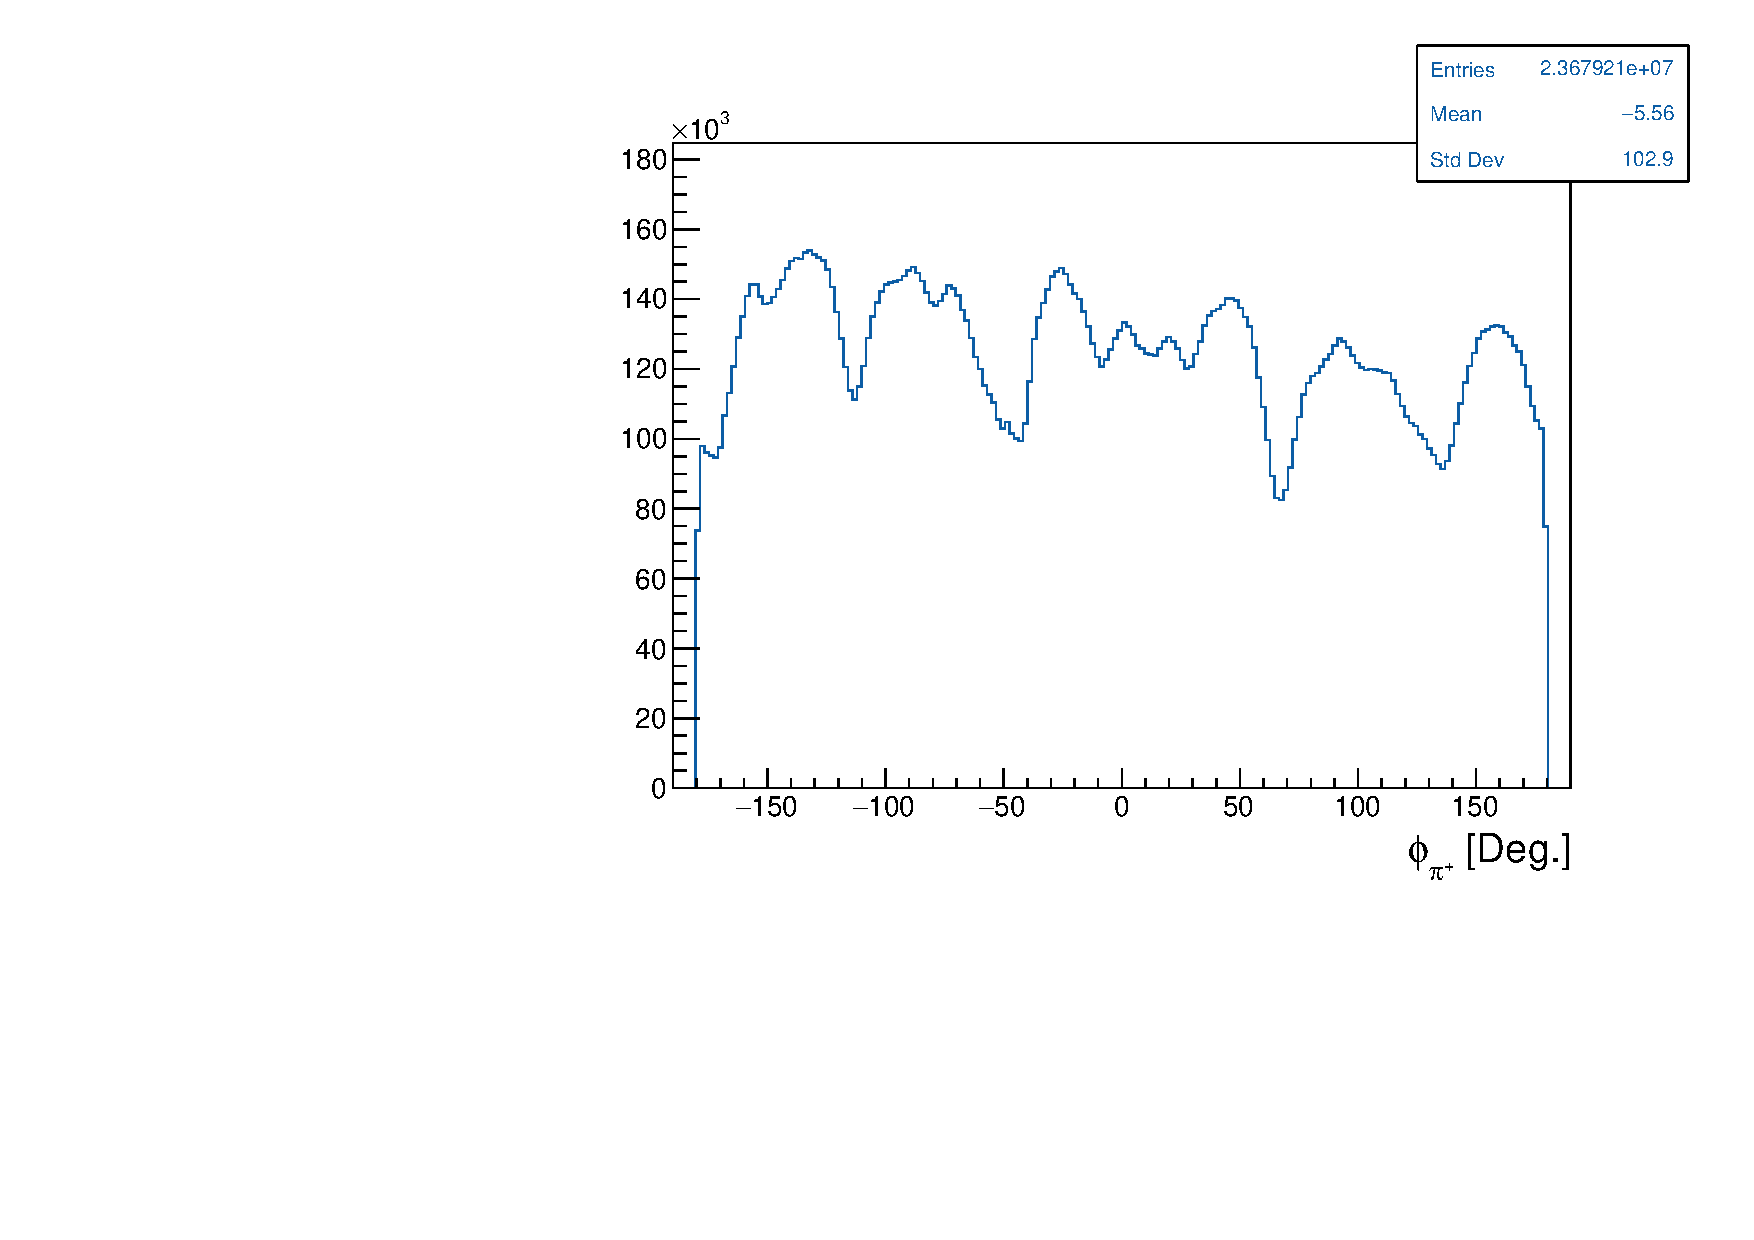
\includegraphics[width=280pt]{/work/clas12/ouillon/Analysis_RG-D/plots_Matt_Study/CxC/electron_kinematics/pdf/phi_e.pdf}
    \end{minipage}

    \begin{minipage}{.5\textwidth}
        \centering
        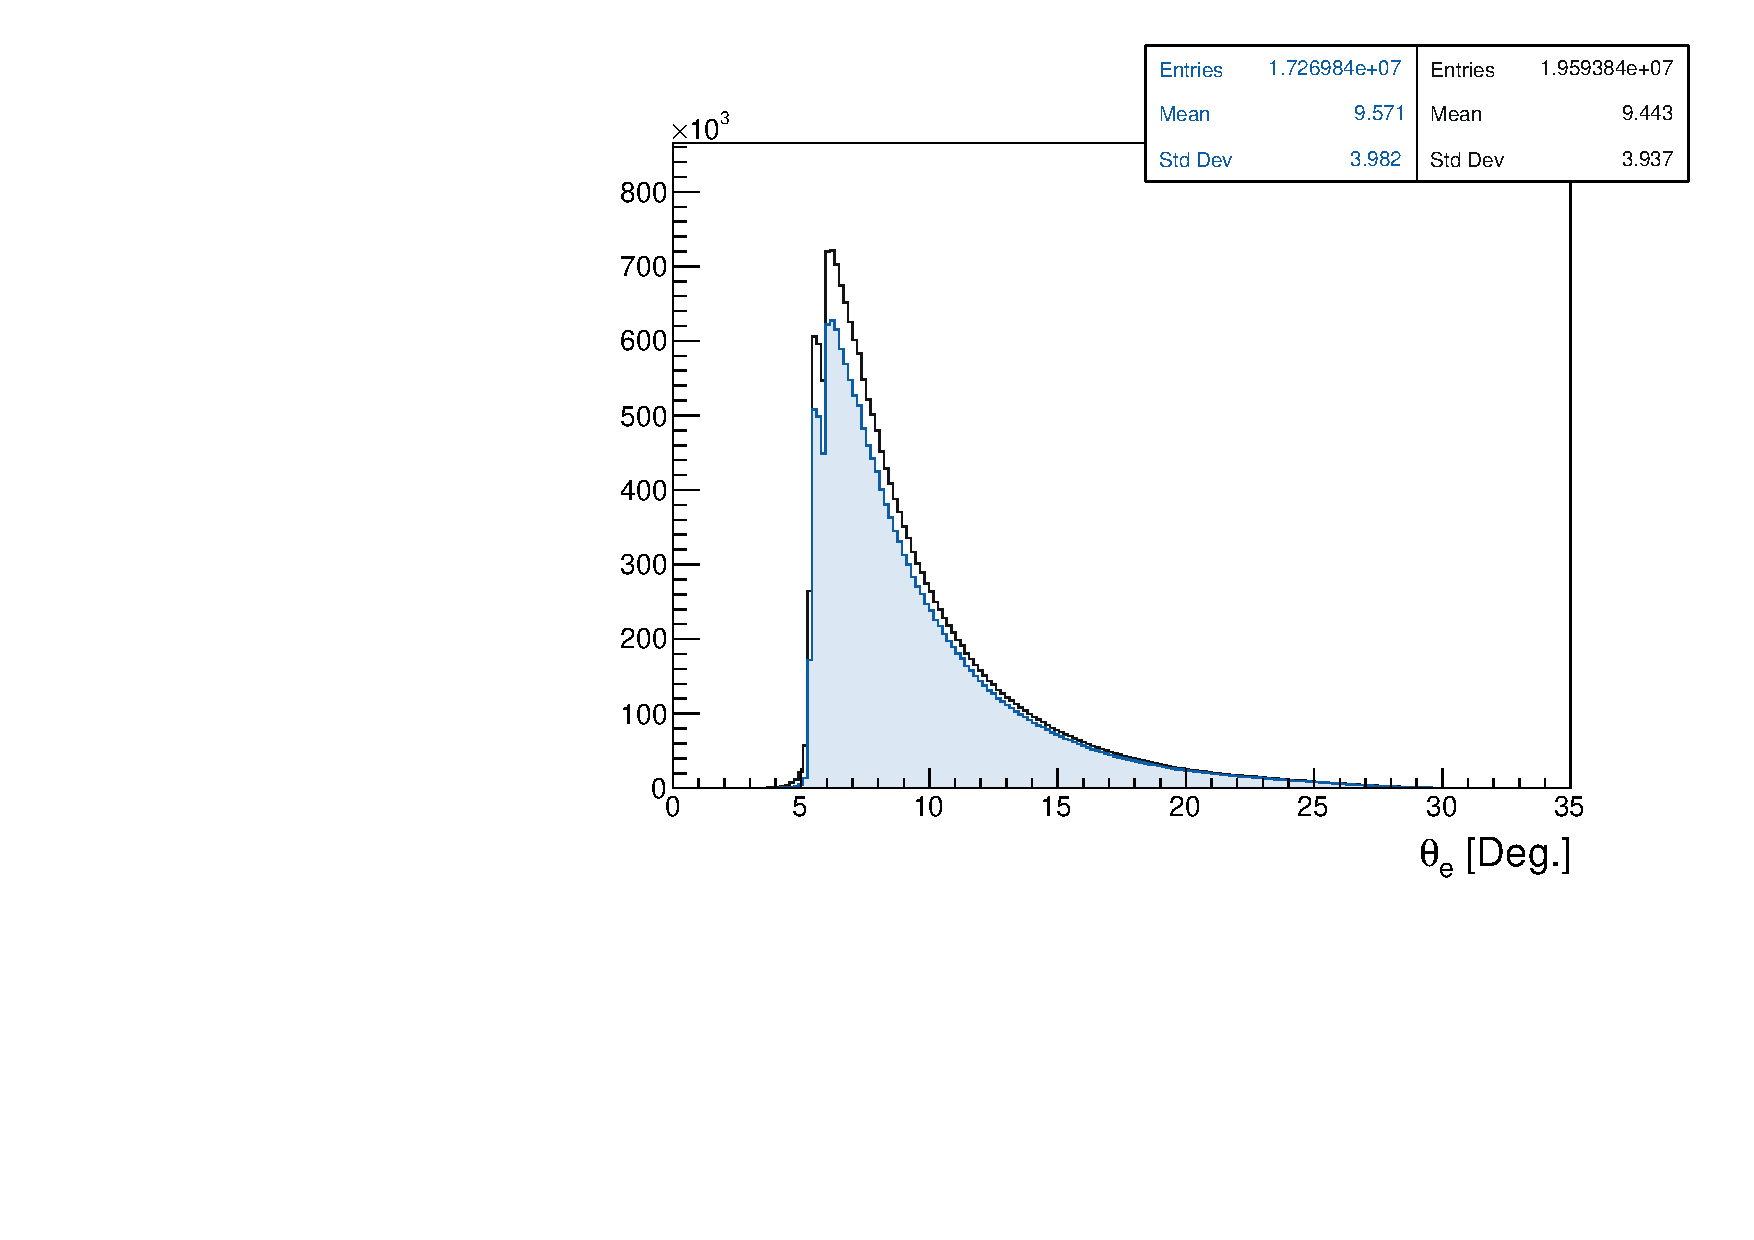
\includegraphics[width=280pt]{/work/clas12/ouillon/Analysis_RG-D/plots_Matt_Study/CxC/electron_kinematics/pdf/theta_e.pdf}
    \end{minipage}
    \begin{minipage}{.5\textwidth}
    \end{minipage}

    \subsection{\(\pi^+\)}
    \begin{minipage}{.5\textwidth}
        \centering
        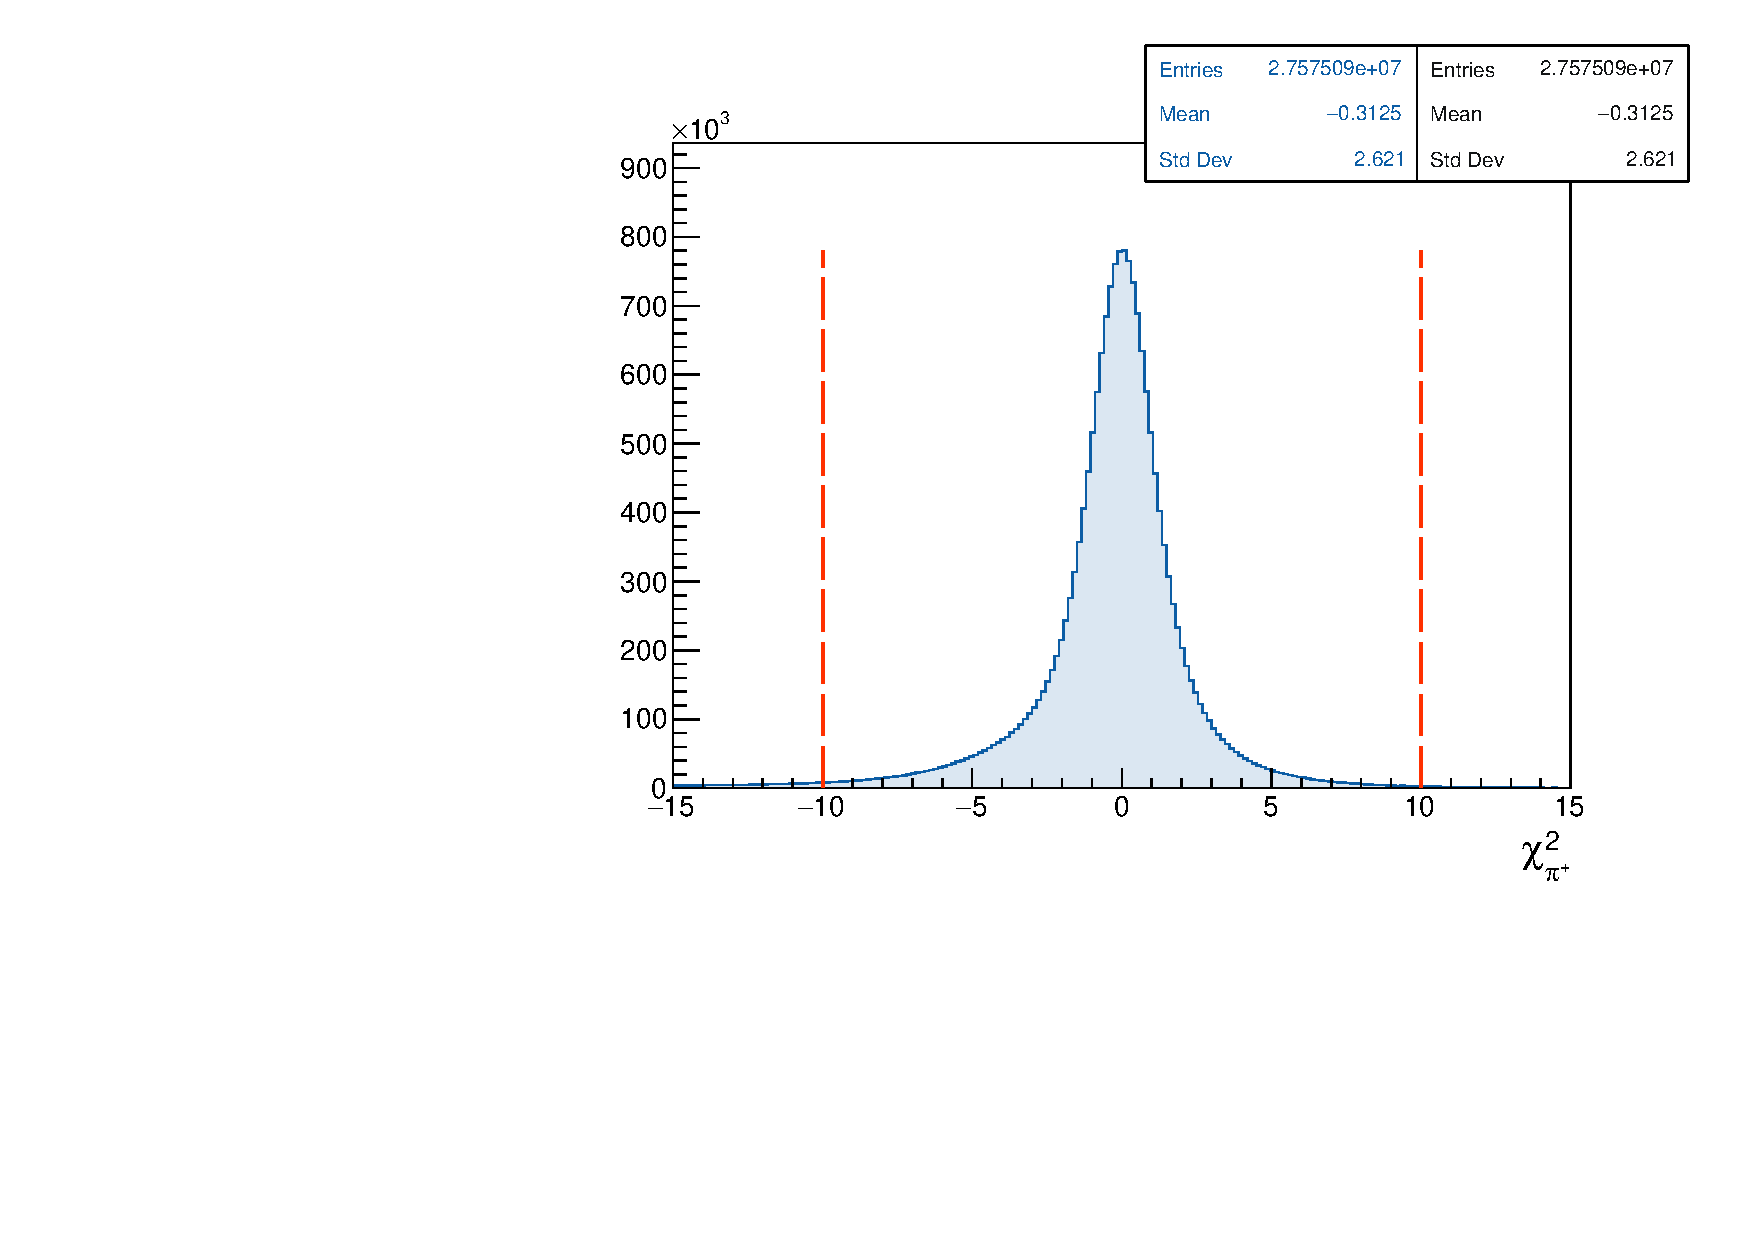
\includegraphics[width=280pt]{/work/clas12/ouillon/Analysis_RG-D/plots_Matt_Study/CxC/allPionPlus_kinematics/pdf/chi2_pion_plus.pdf}
    \end{minipage}
    \begin{minipage}{.5\textwidth}
        \centering
        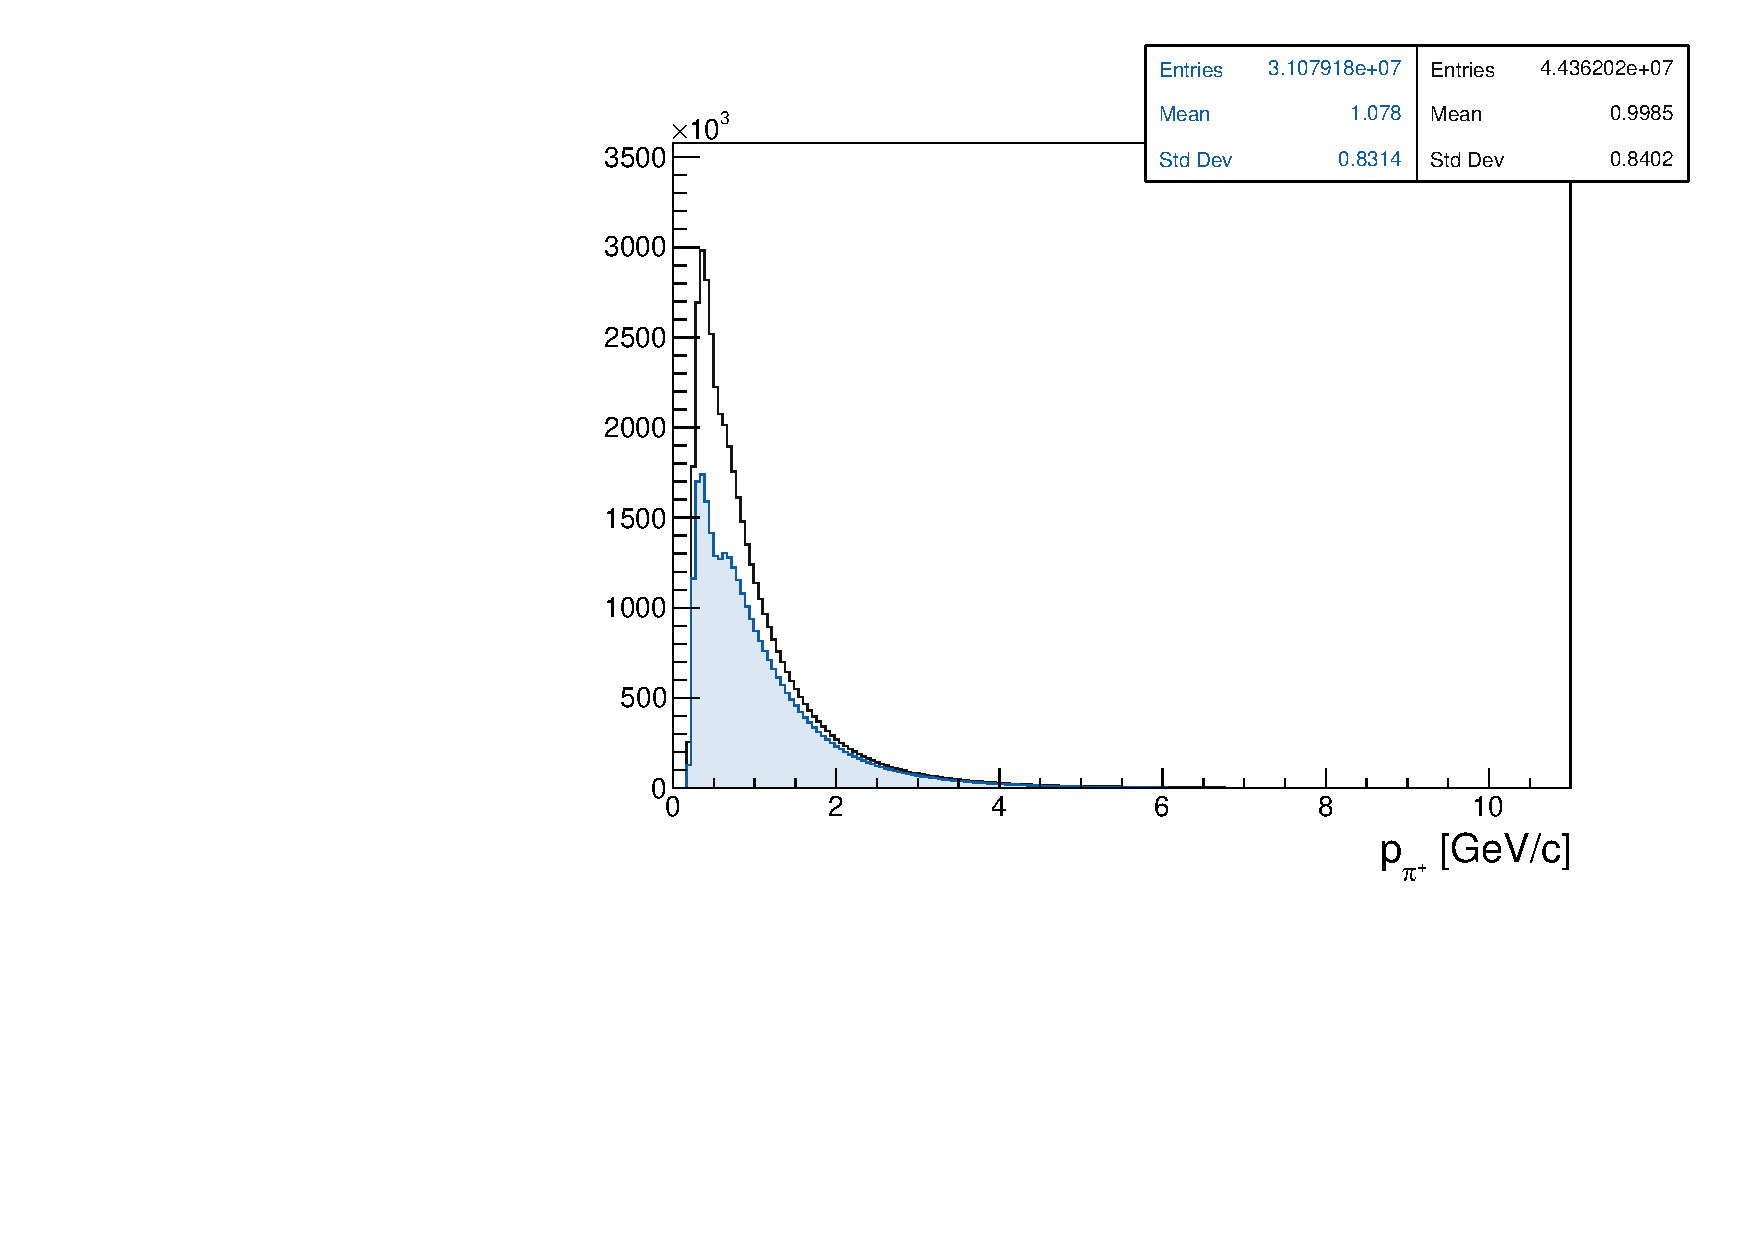
\includegraphics[width=280pt]{/work/clas12/ouillon/Analysis_RG-D/plots_Matt_Study/CxC/allPionPlus_kinematics/pdf/p_pion_plus.pdf}
    \end{minipage}

    \begin{minipage}{.5\textwidth}
        \centering
        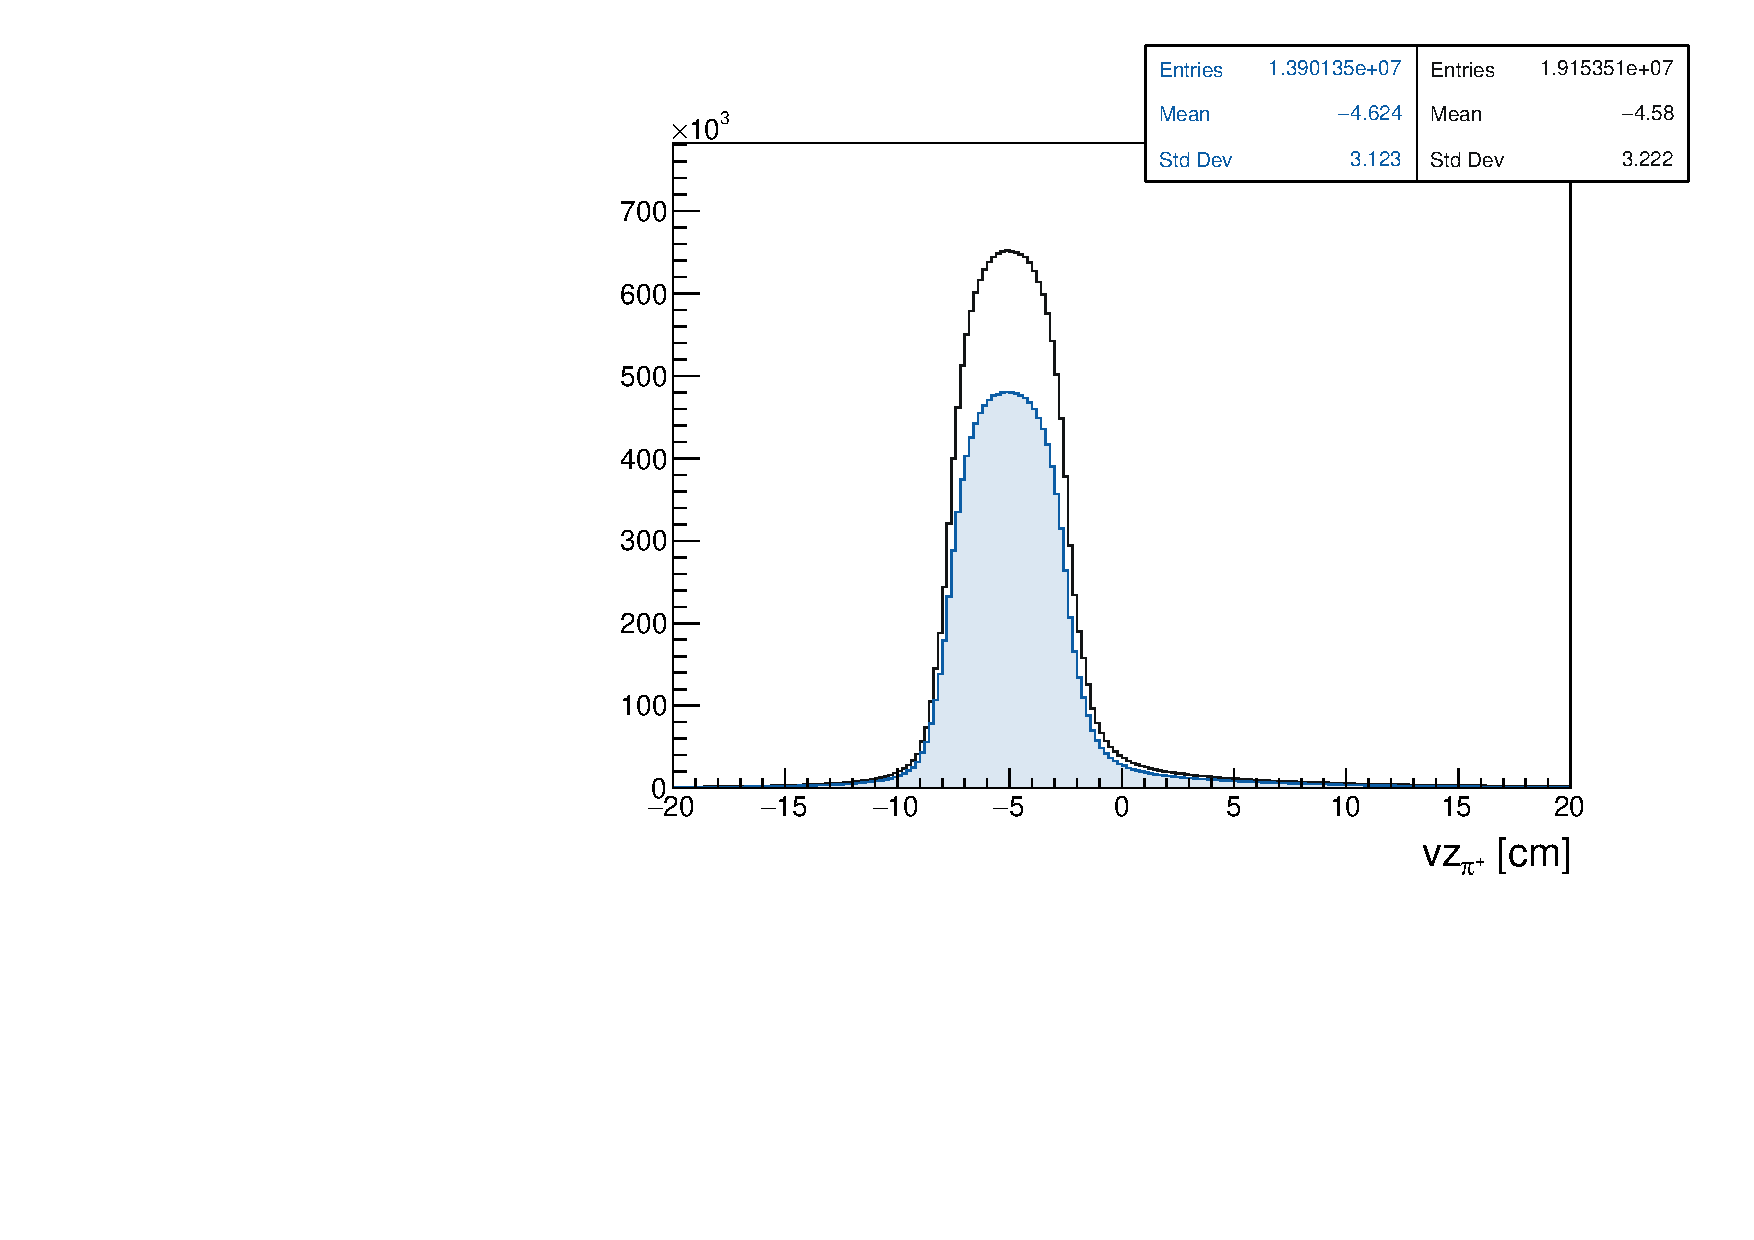
\includegraphics[width=280pt]{/work/clas12/ouillon/Analysis_RG-D/plots_Matt_Study/CxC/allPionPlus_kinematics/pdf/vz_pion_plus.pdf}
    \end{minipage}
    \begin{minipage}{.5\textwidth}
        \centering
        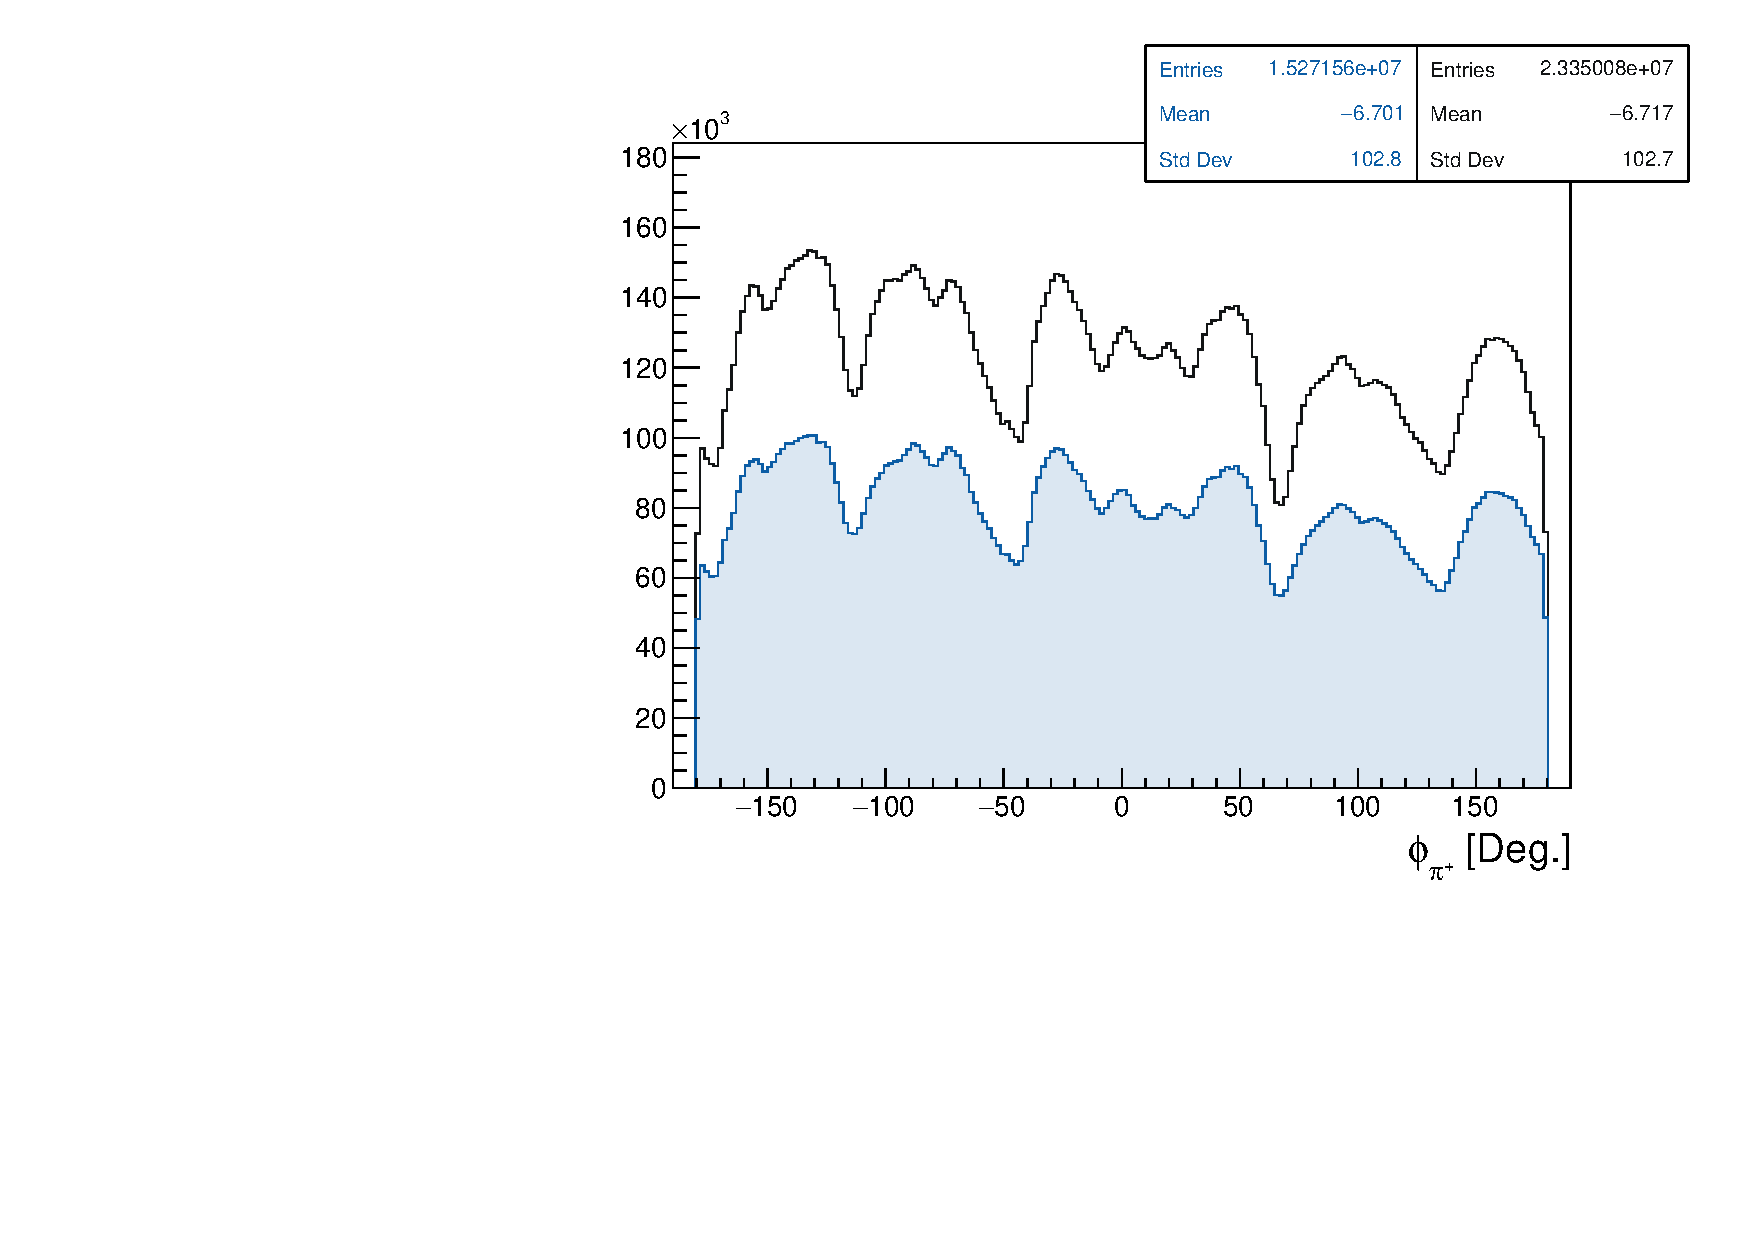
\includegraphics[width=280pt]{/work/clas12/ouillon/Analysis_RG-D/plots_Matt_Study/CxC/allPionPlus_kinematics/pdf/phi_pion_plus.pdf}
    \end{minipage}

    \begin{minipage}{.5\textwidth}
        \centering
        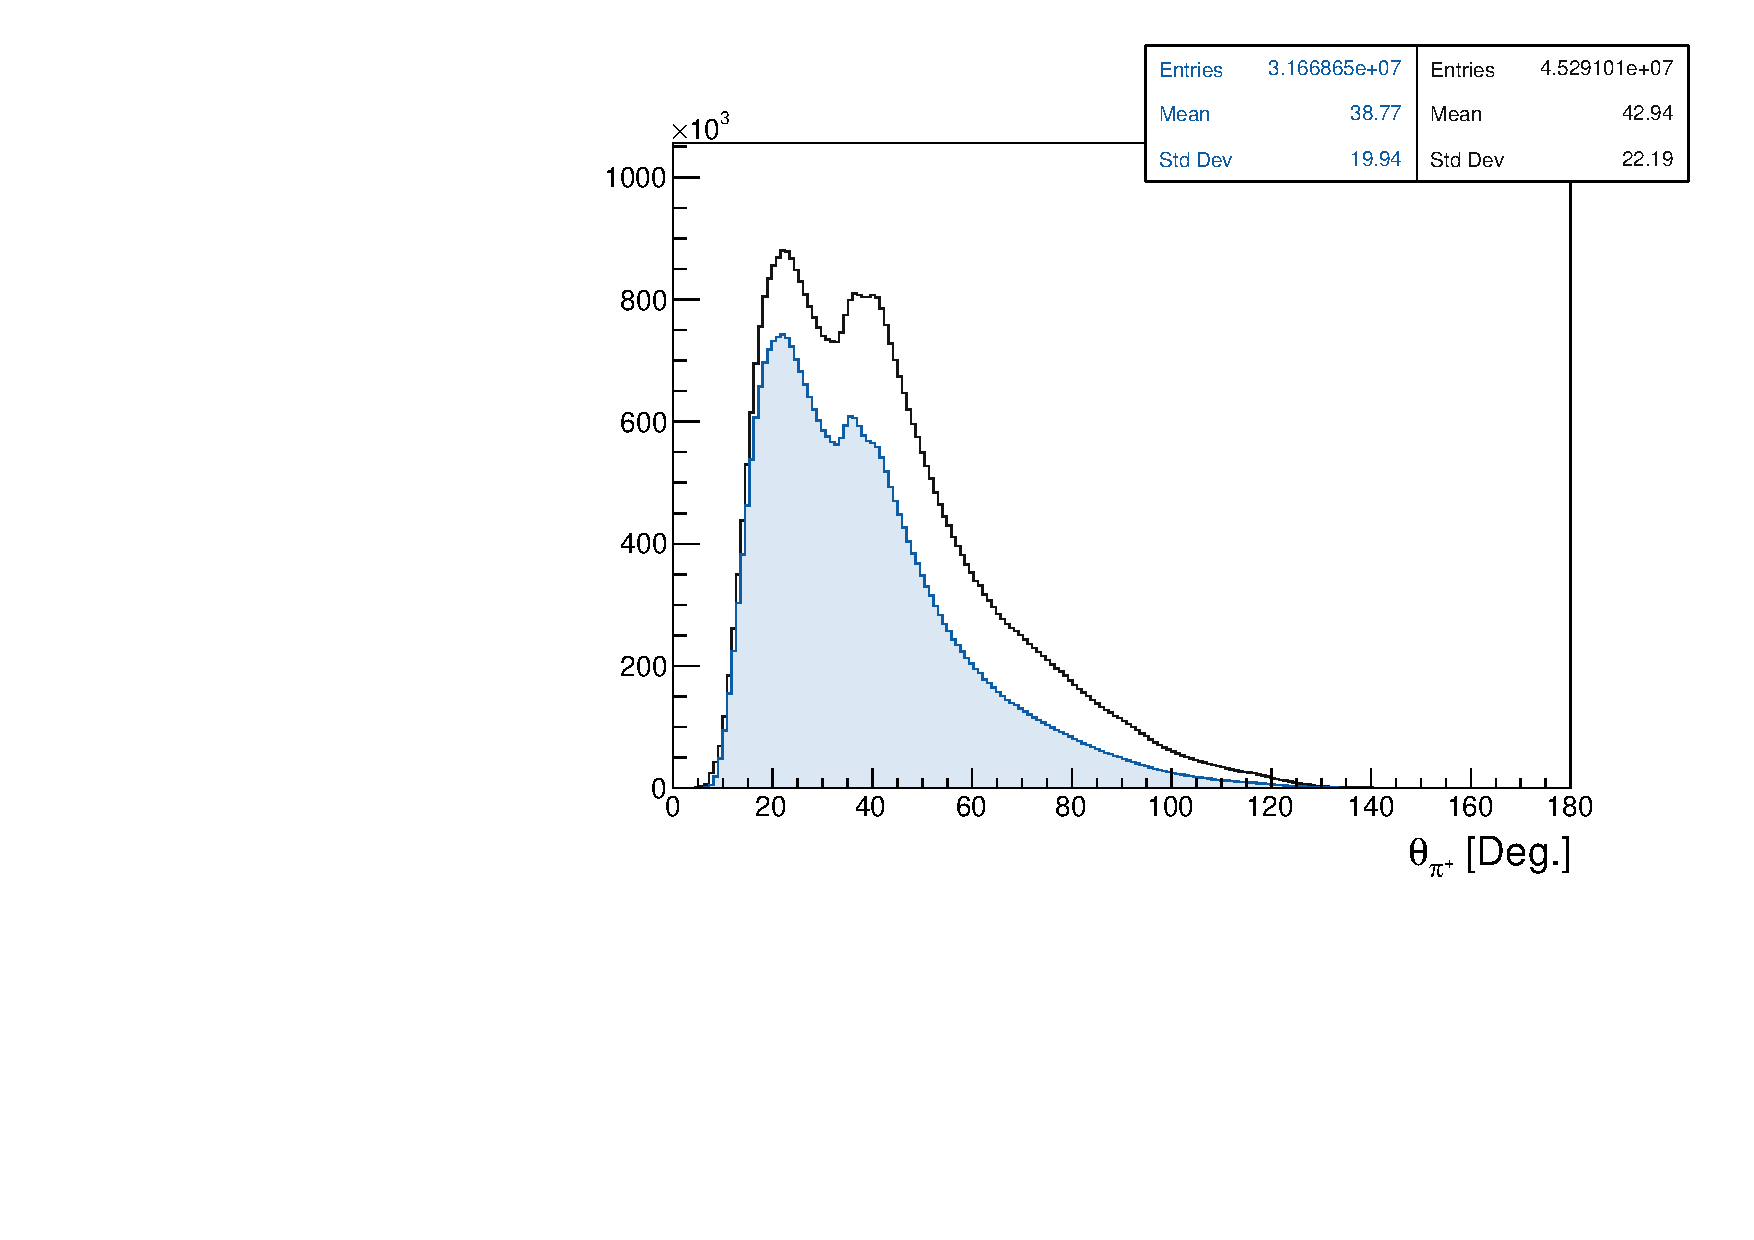
\includegraphics[width=280pt]{/work/clas12/ouillon/Analysis_RG-D/plots_Matt_Study/CxC/allPionPlus_kinematics/pdf/theta_pion_plus.pdf}
    \end{minipage}
    \begin{minipage}{.5\textwidth}
    \end{minipage}

    \subsection{\(\pi^-\)}
    \begin{minipage}{.5\textwidth}
        \centering
        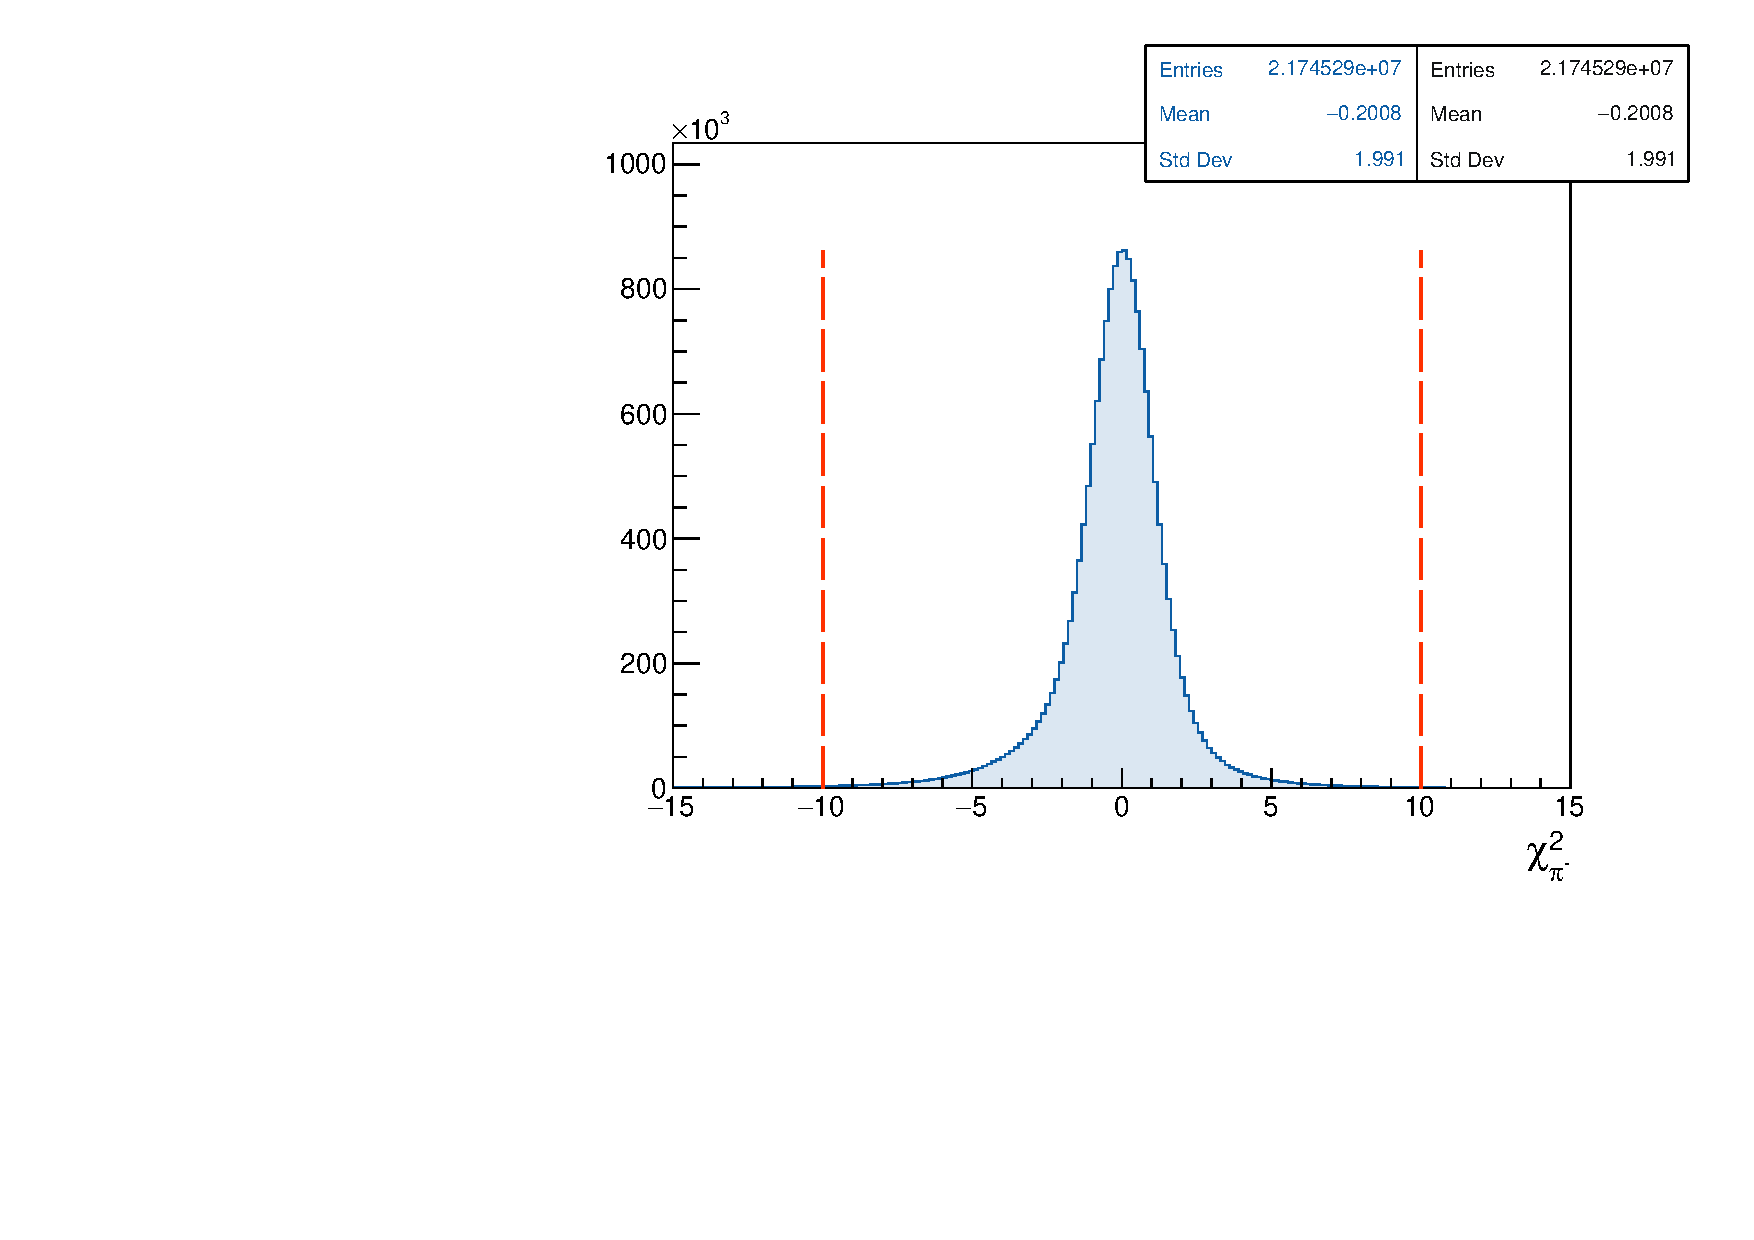
\includegraphics[width=280pt]{/work/clas12/ouillon/Analysis_RG-D/plots_Matt_Study/CxC/allPionMinus_kinematics/pdf/chi2_pion_minus.pdf}
    \end{minipage}
    \begin{minipage}{.5\textwidth}
        \centering
        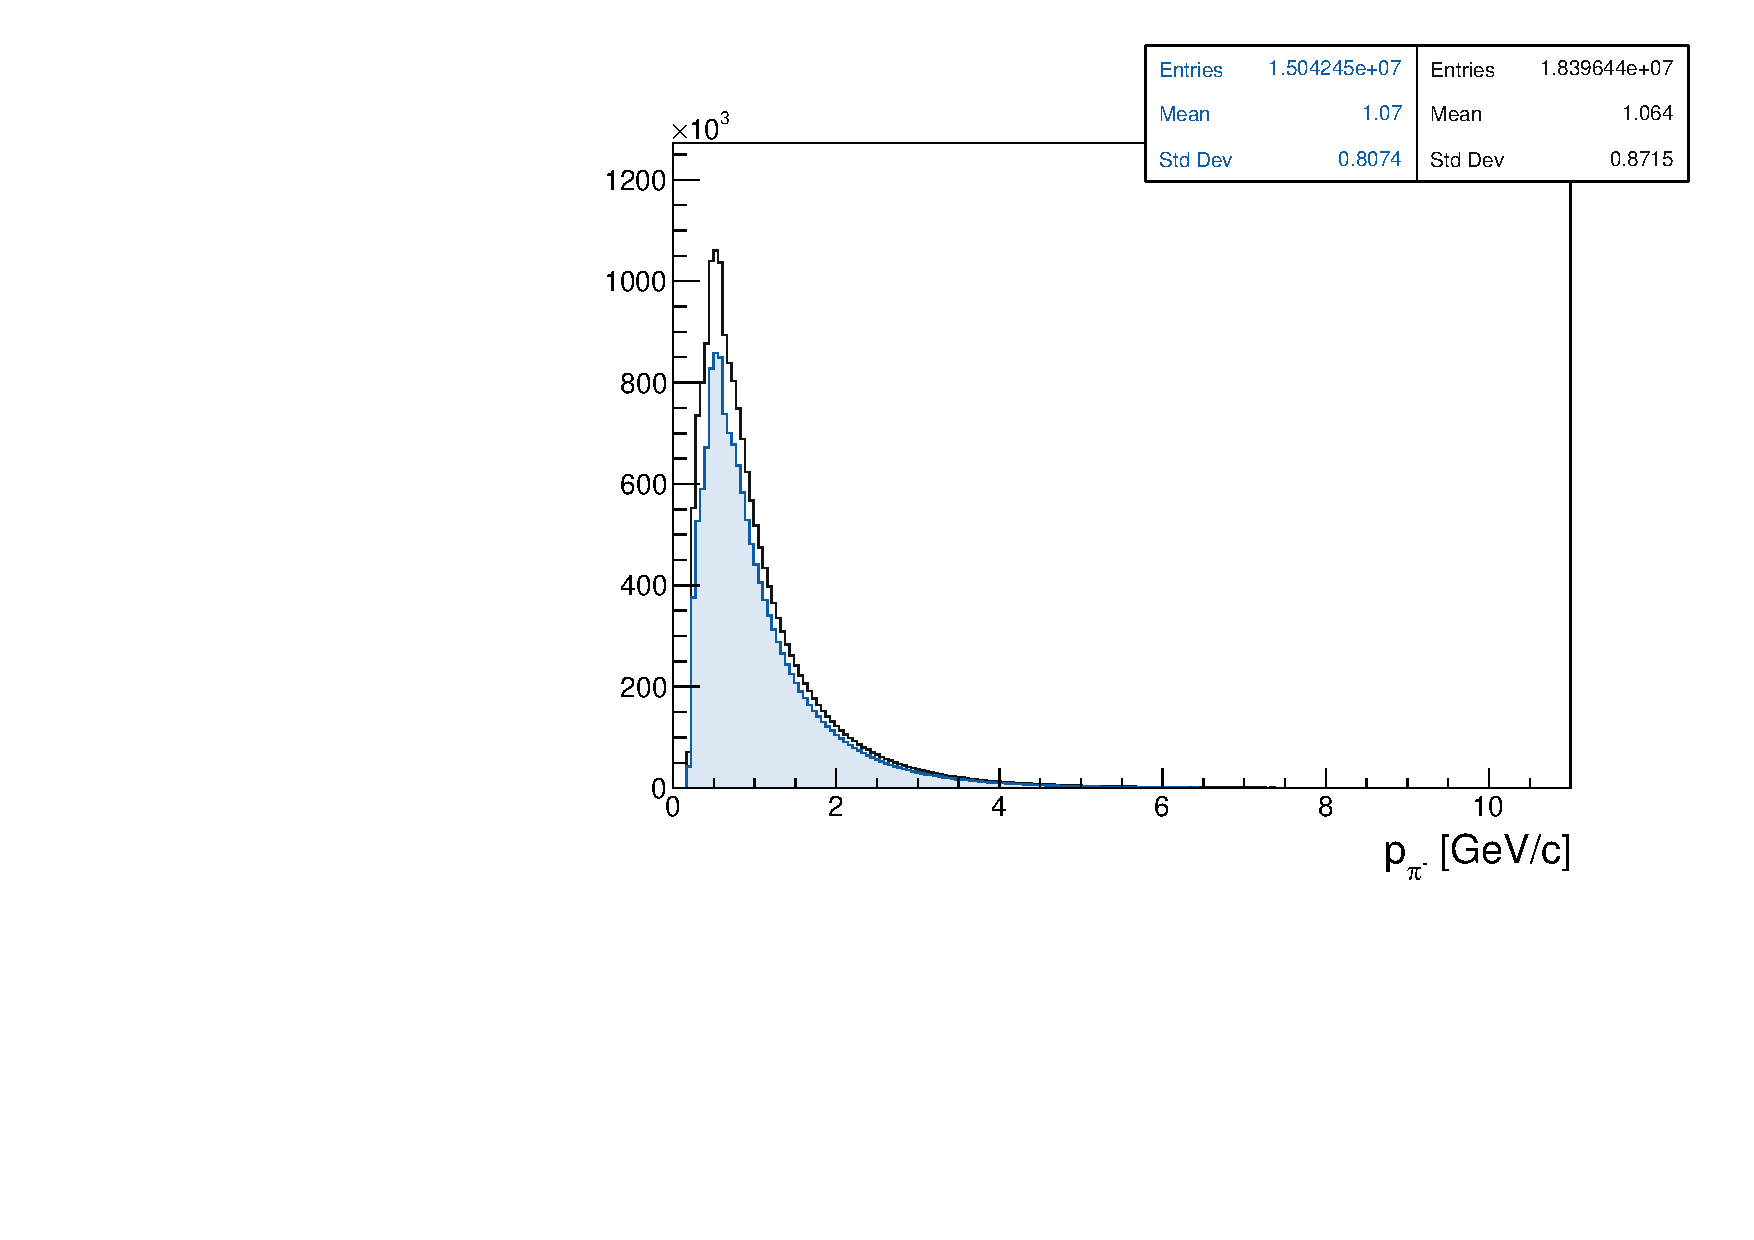
\includegraphics[width=280pt]{/work/clas12/ouillon/Analysis_RG-D/plots_Matt_Study/CxC/allPionMinus_kinematics/pdf/p_pion_minus.pdf}
    \end{minipage}

    \begin{minipage}{.5\textwidth}
        \centering
        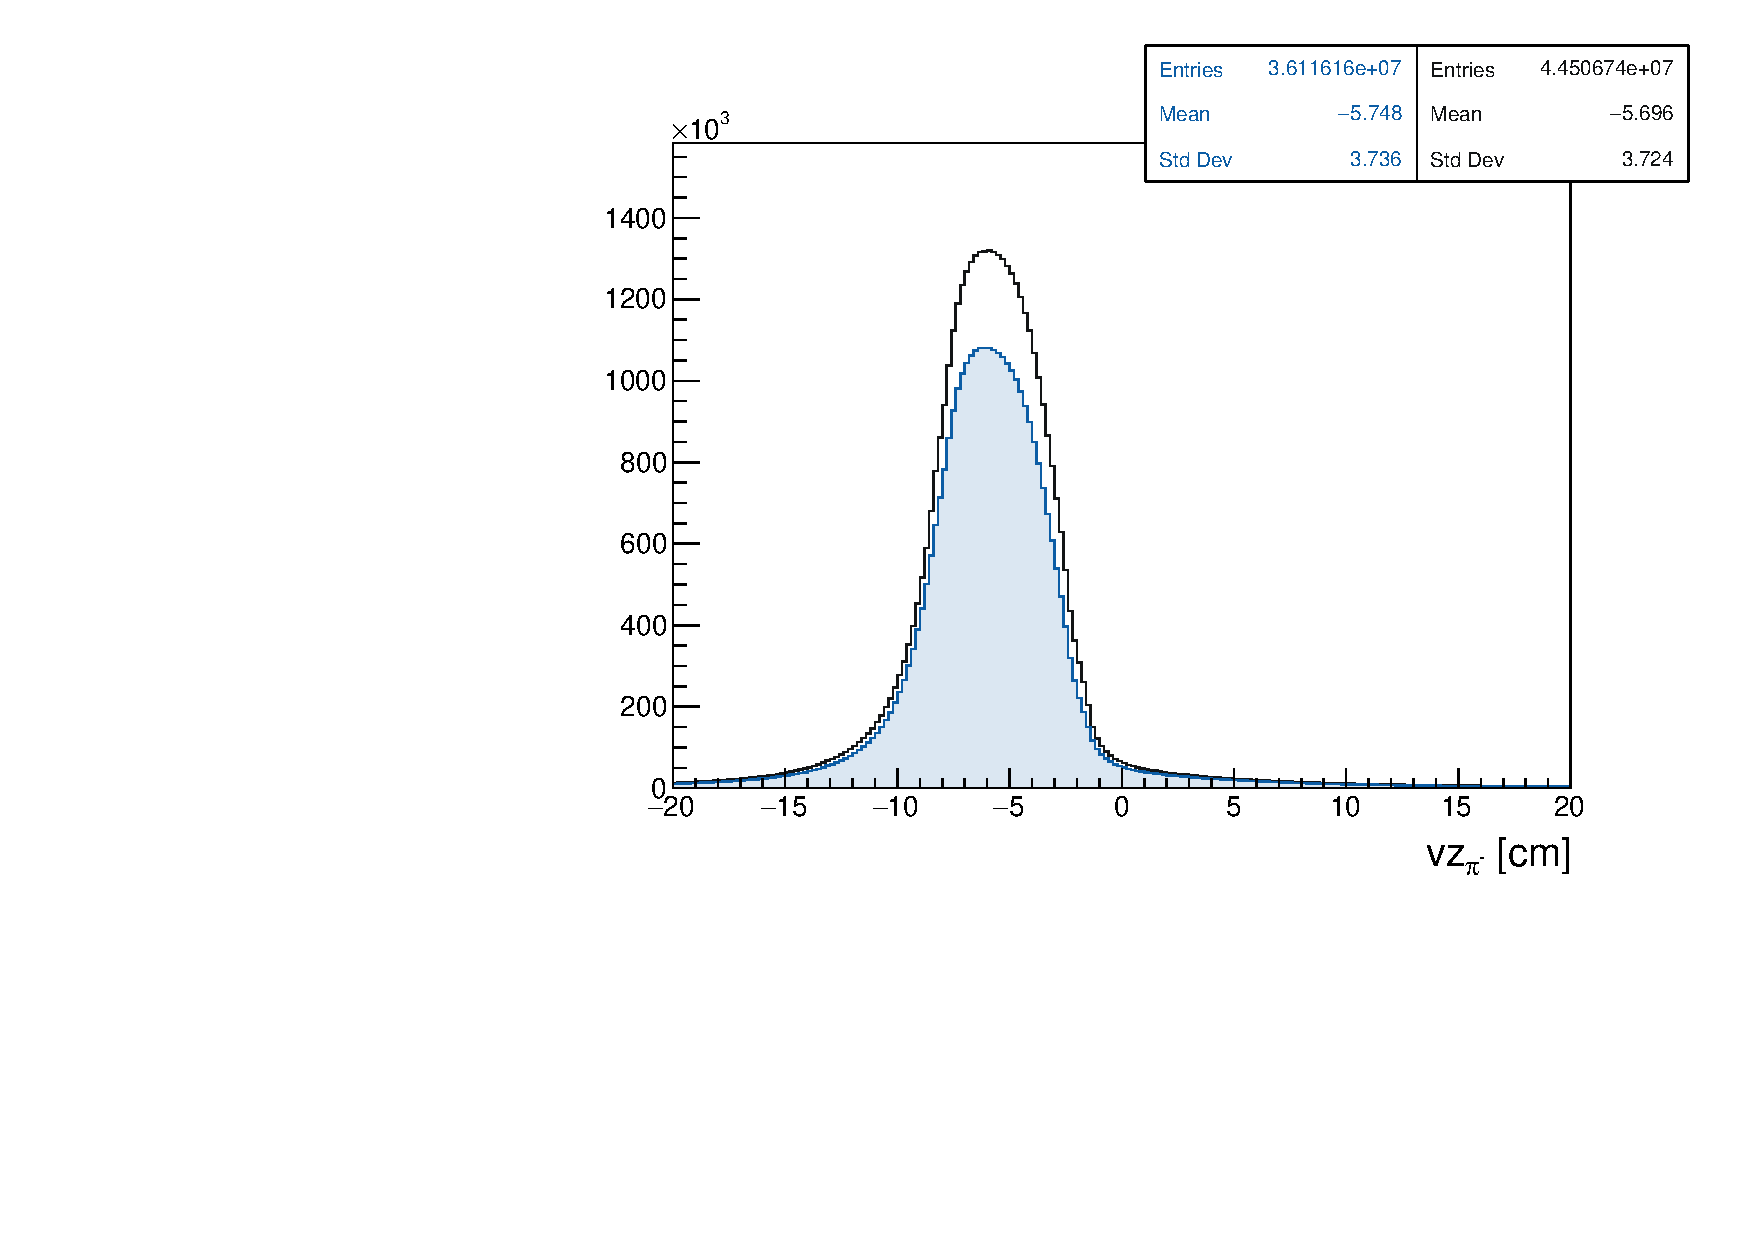
\includegraphics[width=280pt]{/work/clas12/ouillon/Analysis_RG-D/plots_Matt_Study/CxC/allPionMinus_kinematics/pdf/vz_pion_minus.pdf}
    \end{minipage}
    \begin{minipage}{.5\textwidth}
        \centering
        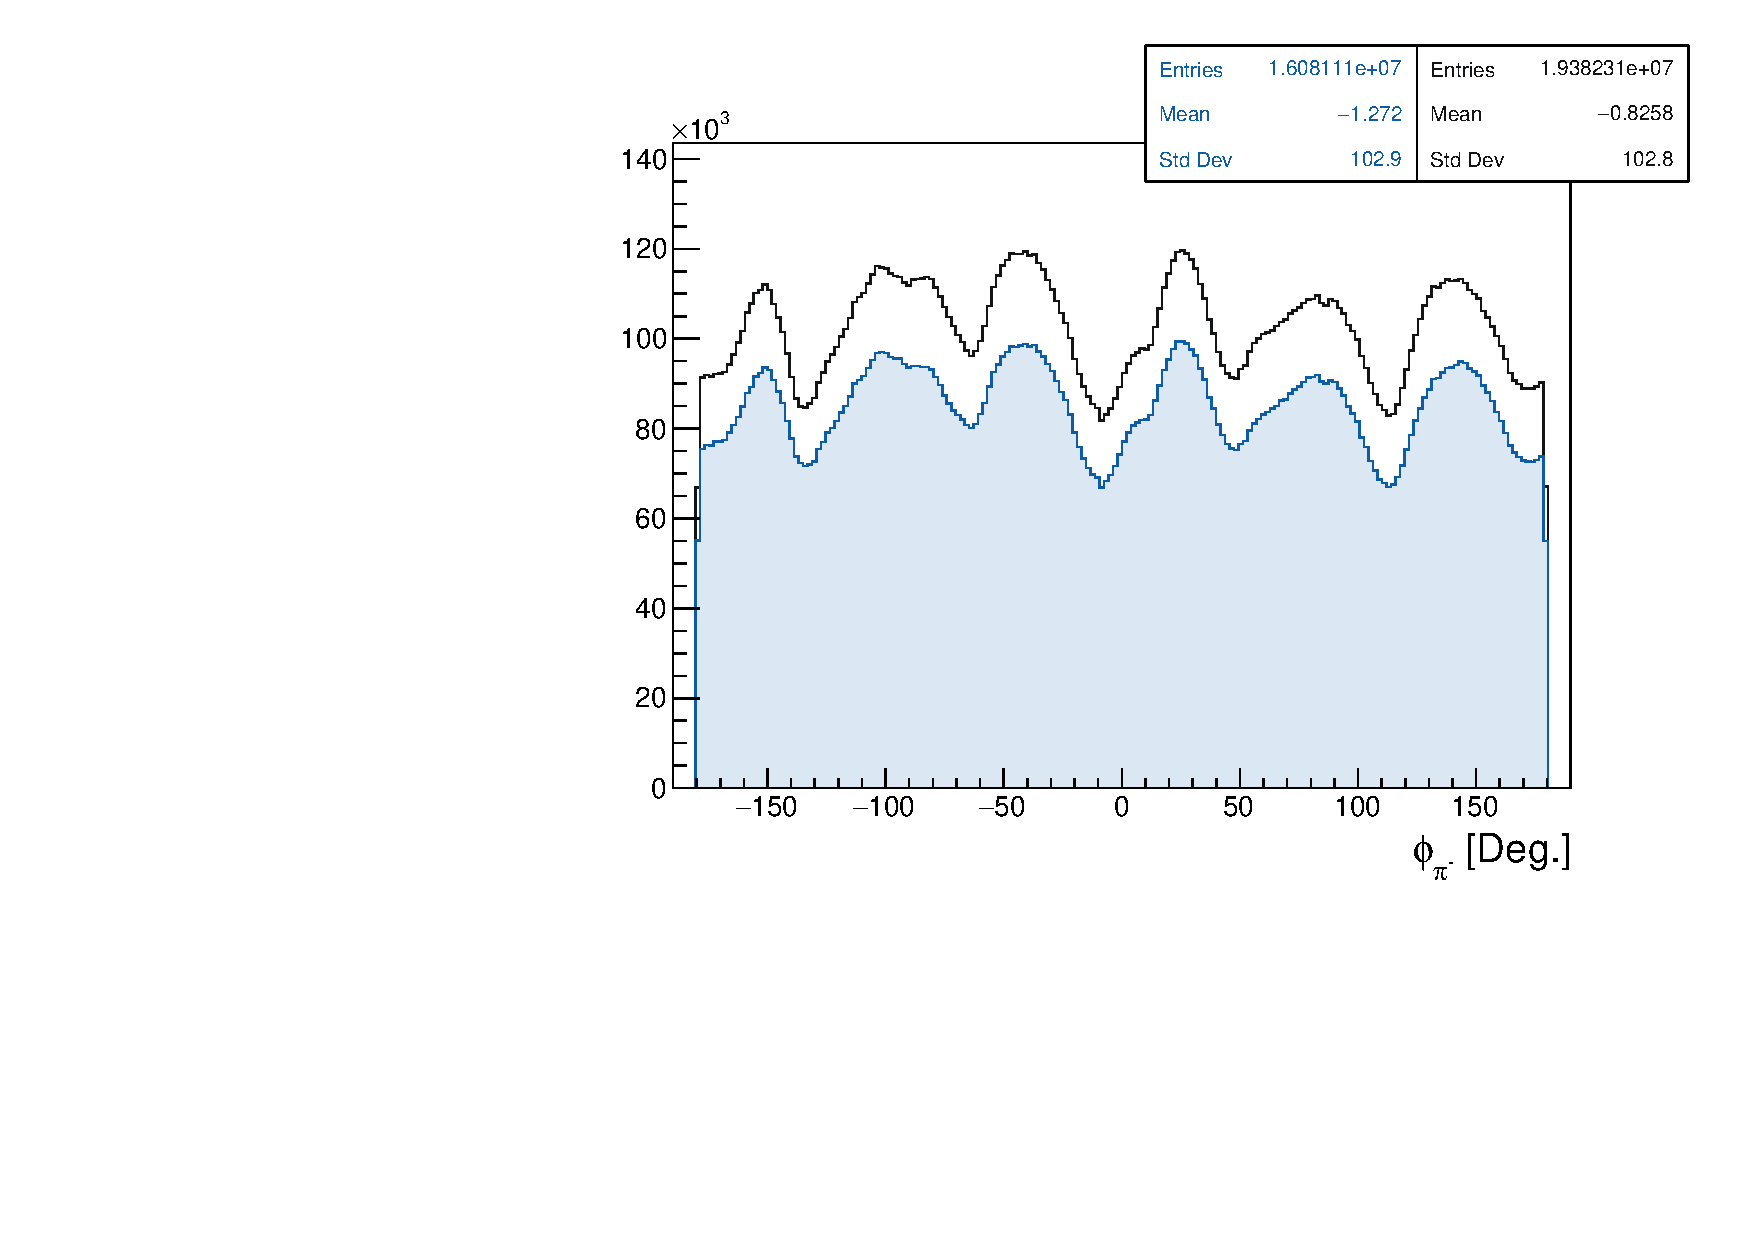
\includegraphics[width=280pt]{/work/clas12/ouillon/Analysis_RG-D/plots_Matt_Study/CxC/allPionMinus_kinematics/pdf/phi_pion_minus.pdf}
    \end{minipage}

    \begin{minipage}{.5\textwidth}
        \centering
        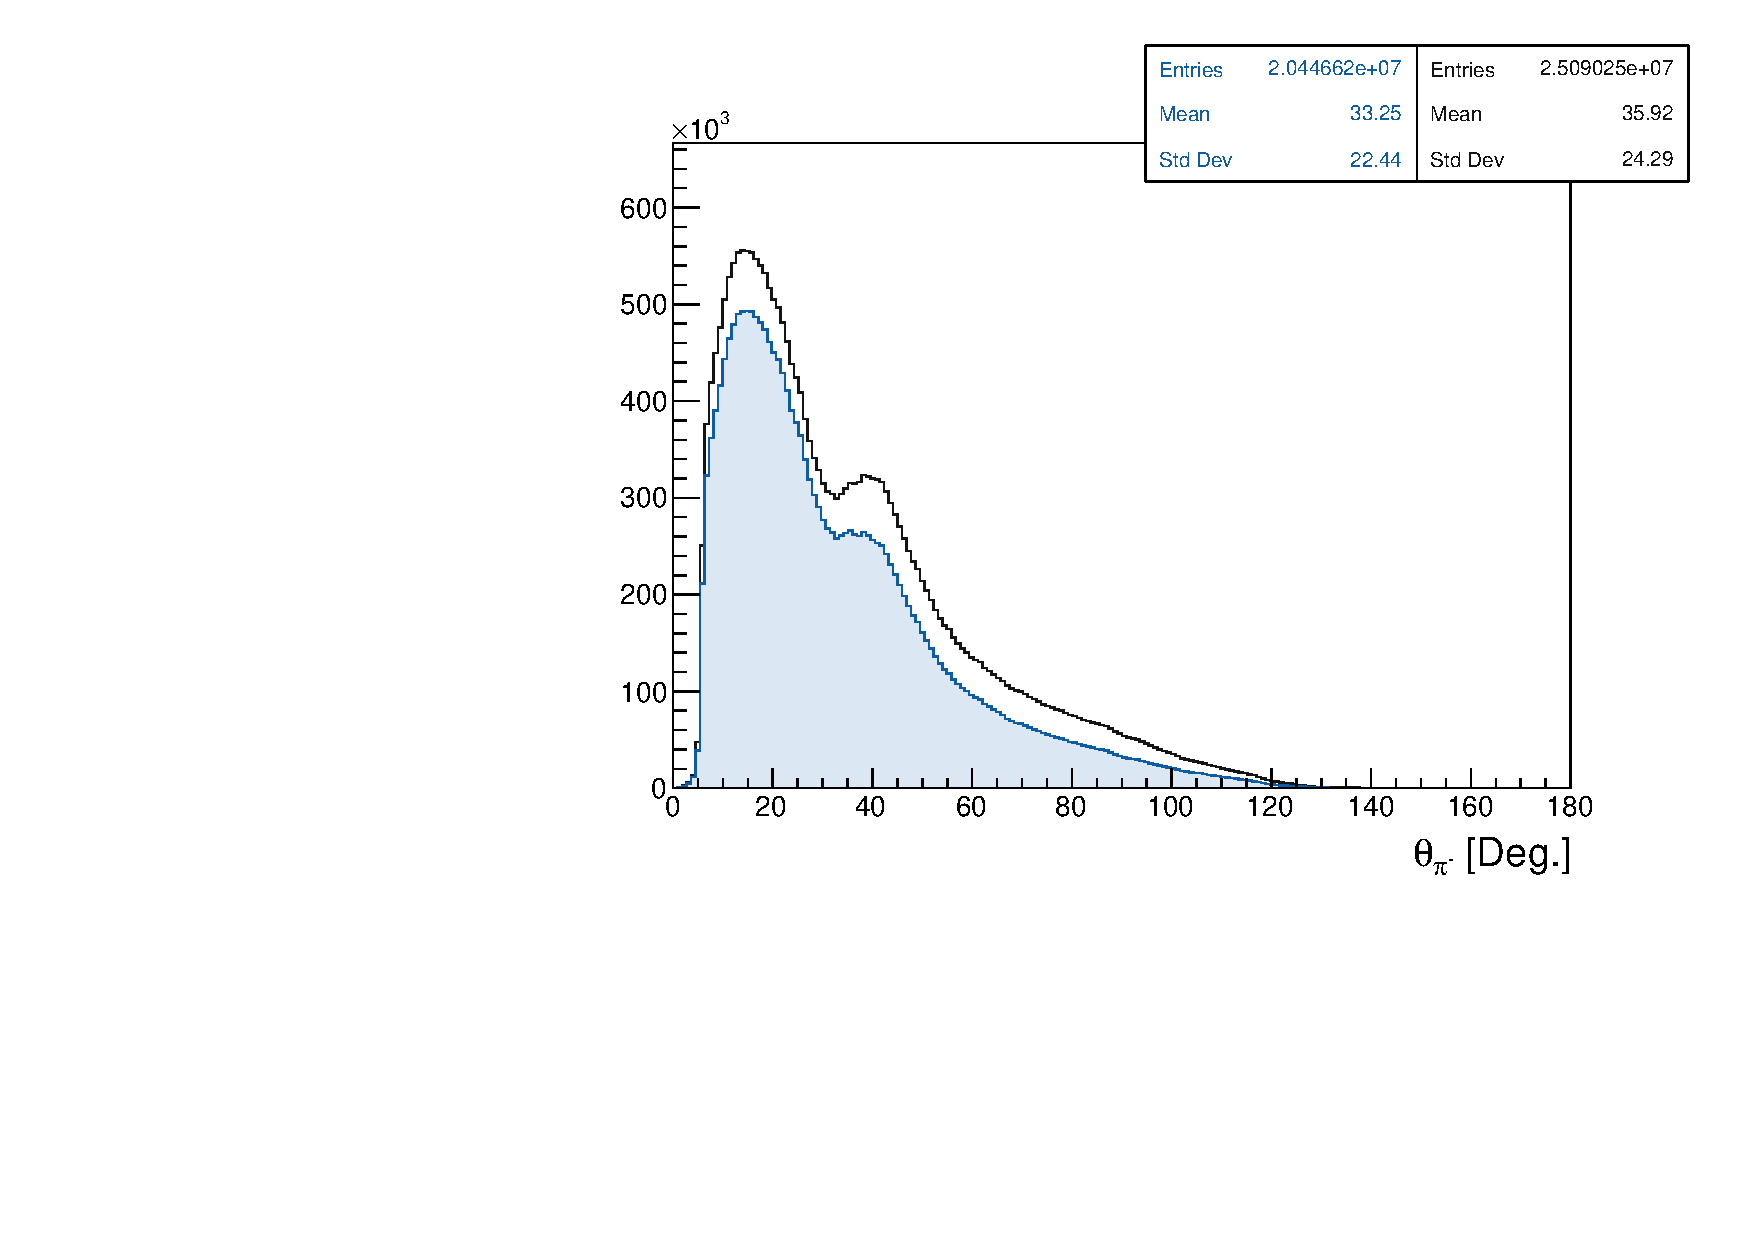
\includegraphics[width=280pt]{/work/clas12/ouillon/Analysis_RG-D/plots_Matt_Study/CxC/allPionMinus_kinematics/pdf/theta_pion_minus.pdf}
    \end{minipage}
    \begin{minipage}{.5\textwidth}
    \end{minipage}

    \subsection{Event selection}
    \begin{minipage}{.5\textwidth}
        \centering
        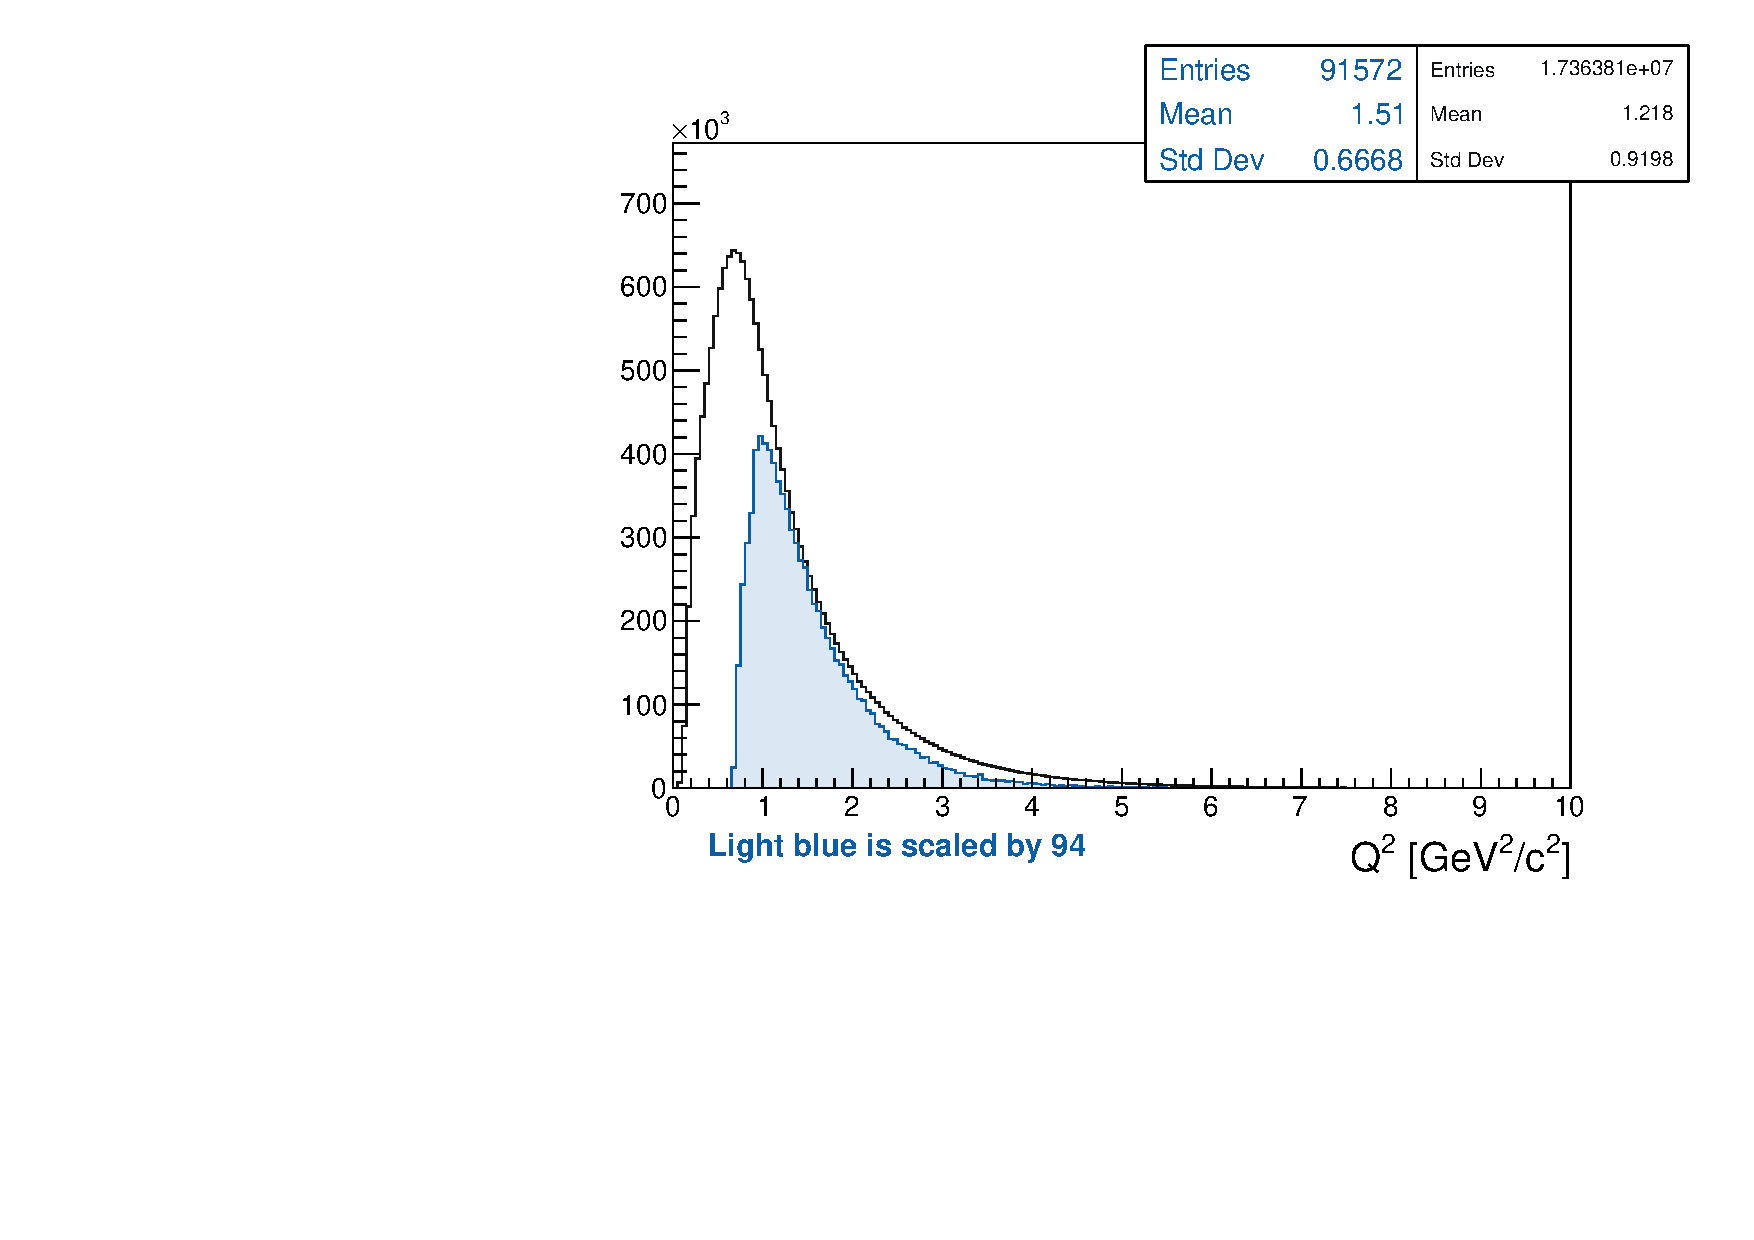
\includegraphics[width=280pt]{/work/clas12/ouillon/Analysis_RG-D/plots_Matt_Study/CxC/event_kinematics/pdf/Q2.pdf}
    \end{minipage}
    \begin{minipage}{.5\textwidth}
        \centering
        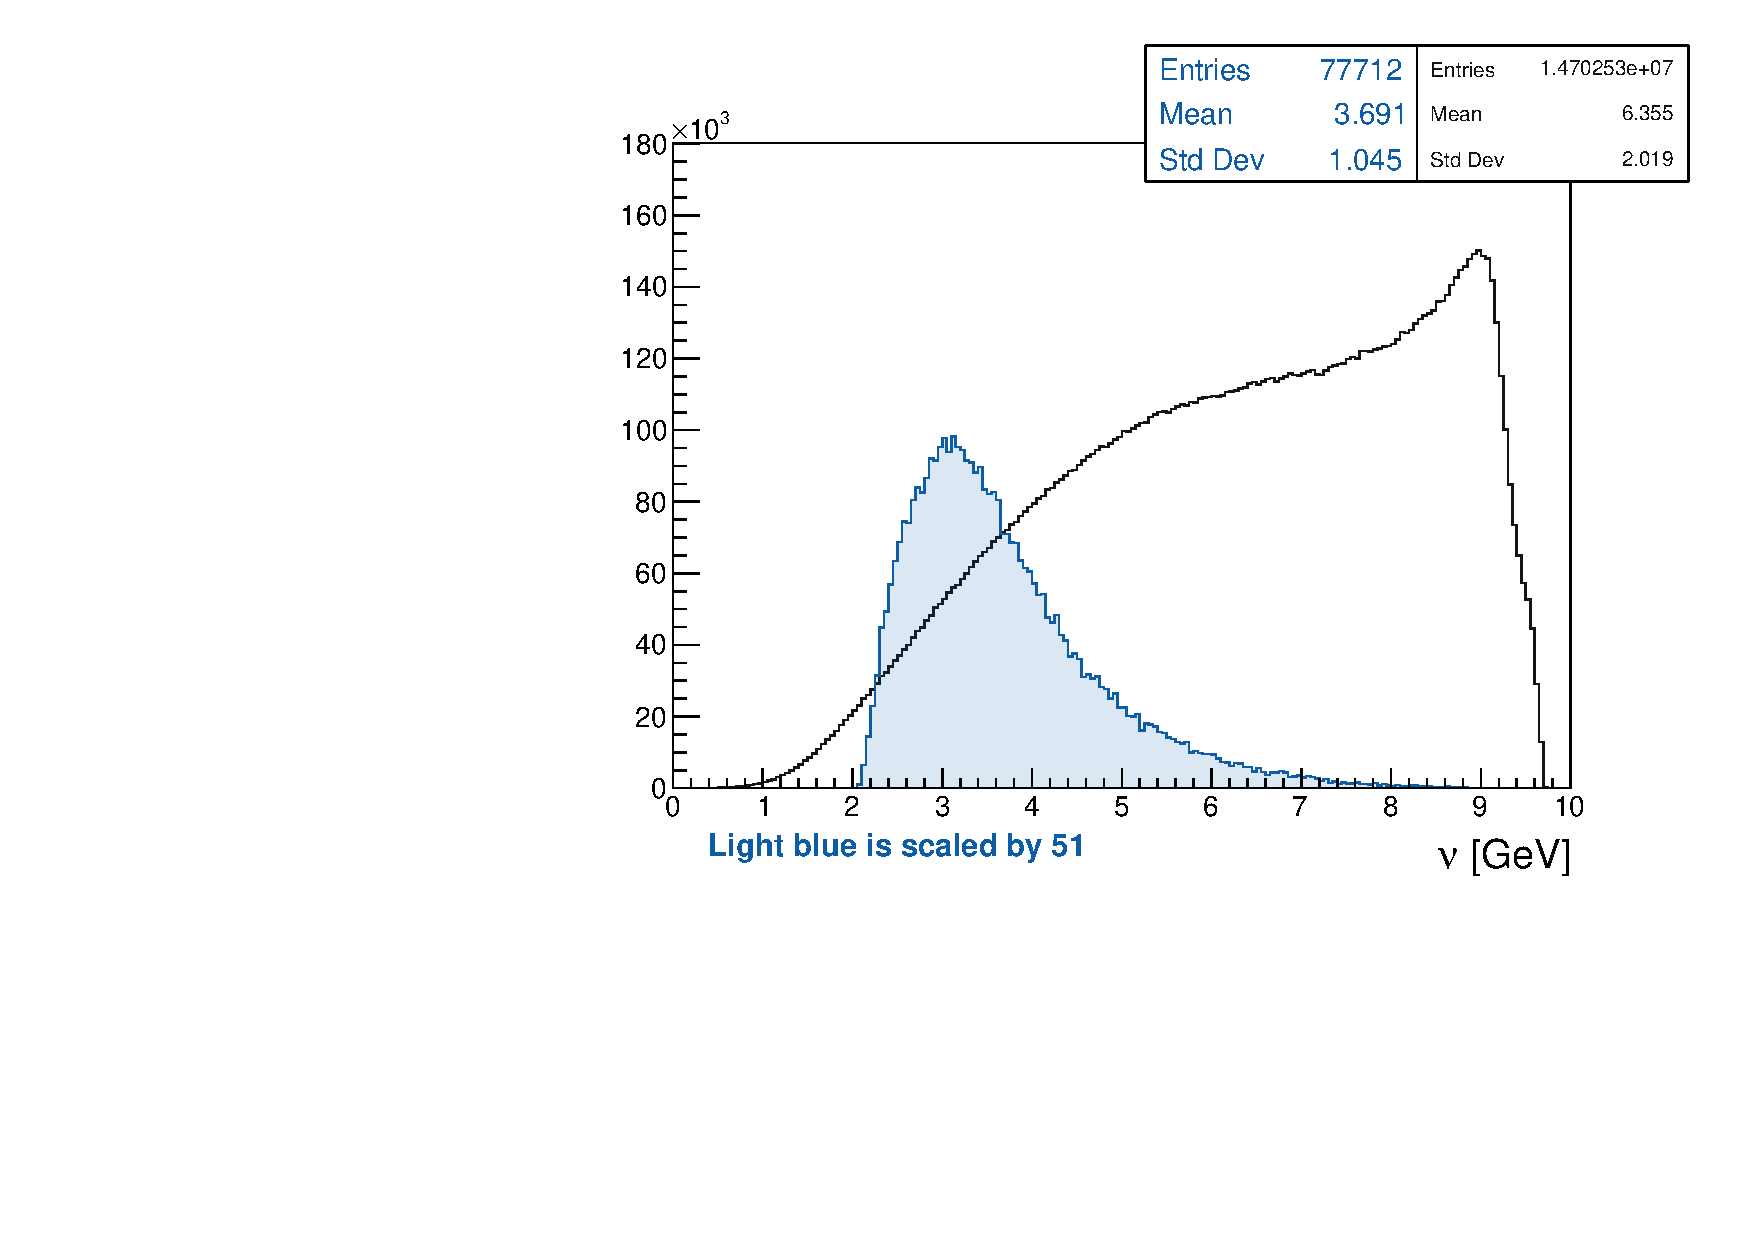
\includegraphics[width=280pt]{/work/clas12/ouillon/Analysis_RG-D/plots_Matt_Study/CxC/event_kinematics/pdf/nu.pdf}
    \end{minipage}

    \begin{minipage}{.5\textwidth}
        \centering
        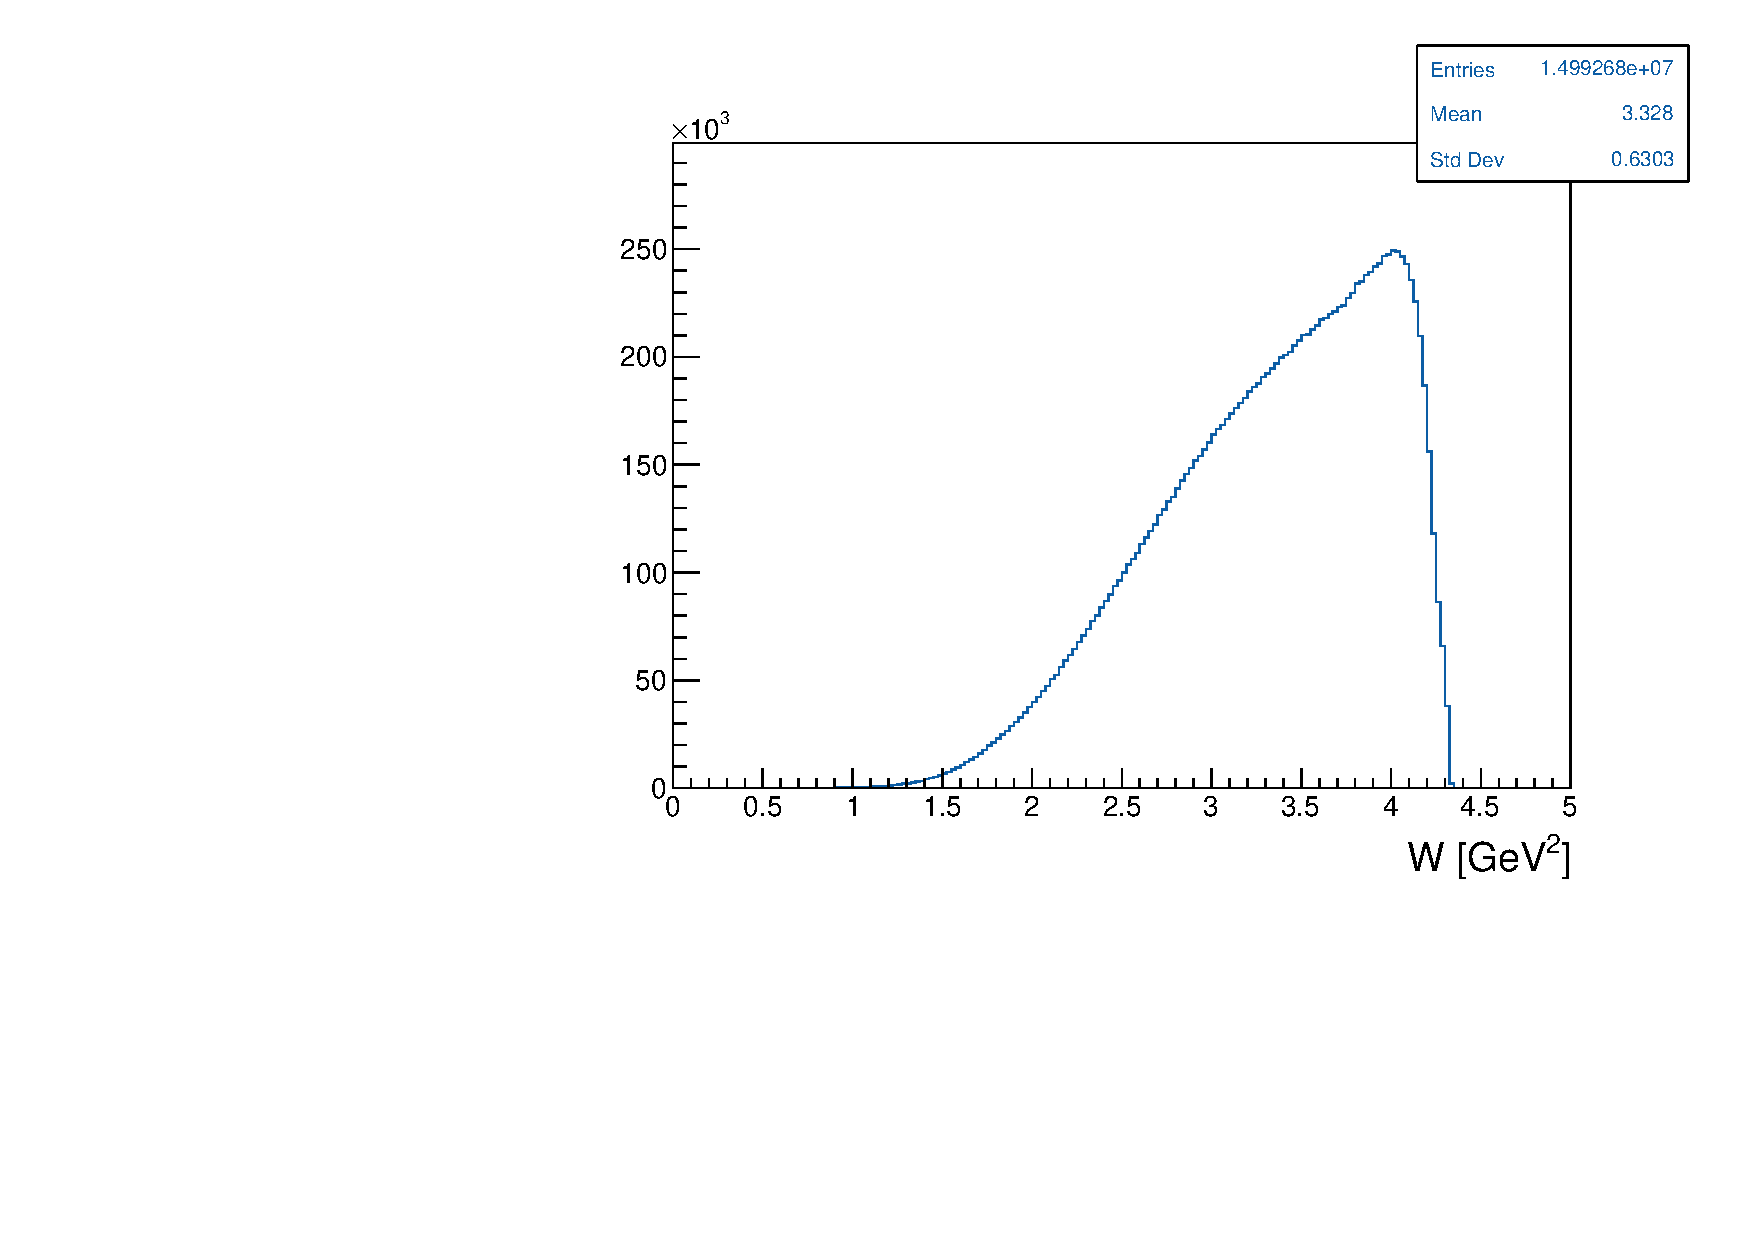
\includegraphics[width=280pt]{/work/clas12/ouillon/Analysis_RG-D/plots_Matt_Study/CxC/event_kinematics/pdf/W.pdf}
    \end{minipage}
    \begin{minipage}{.5\textwidth}
        \centering
        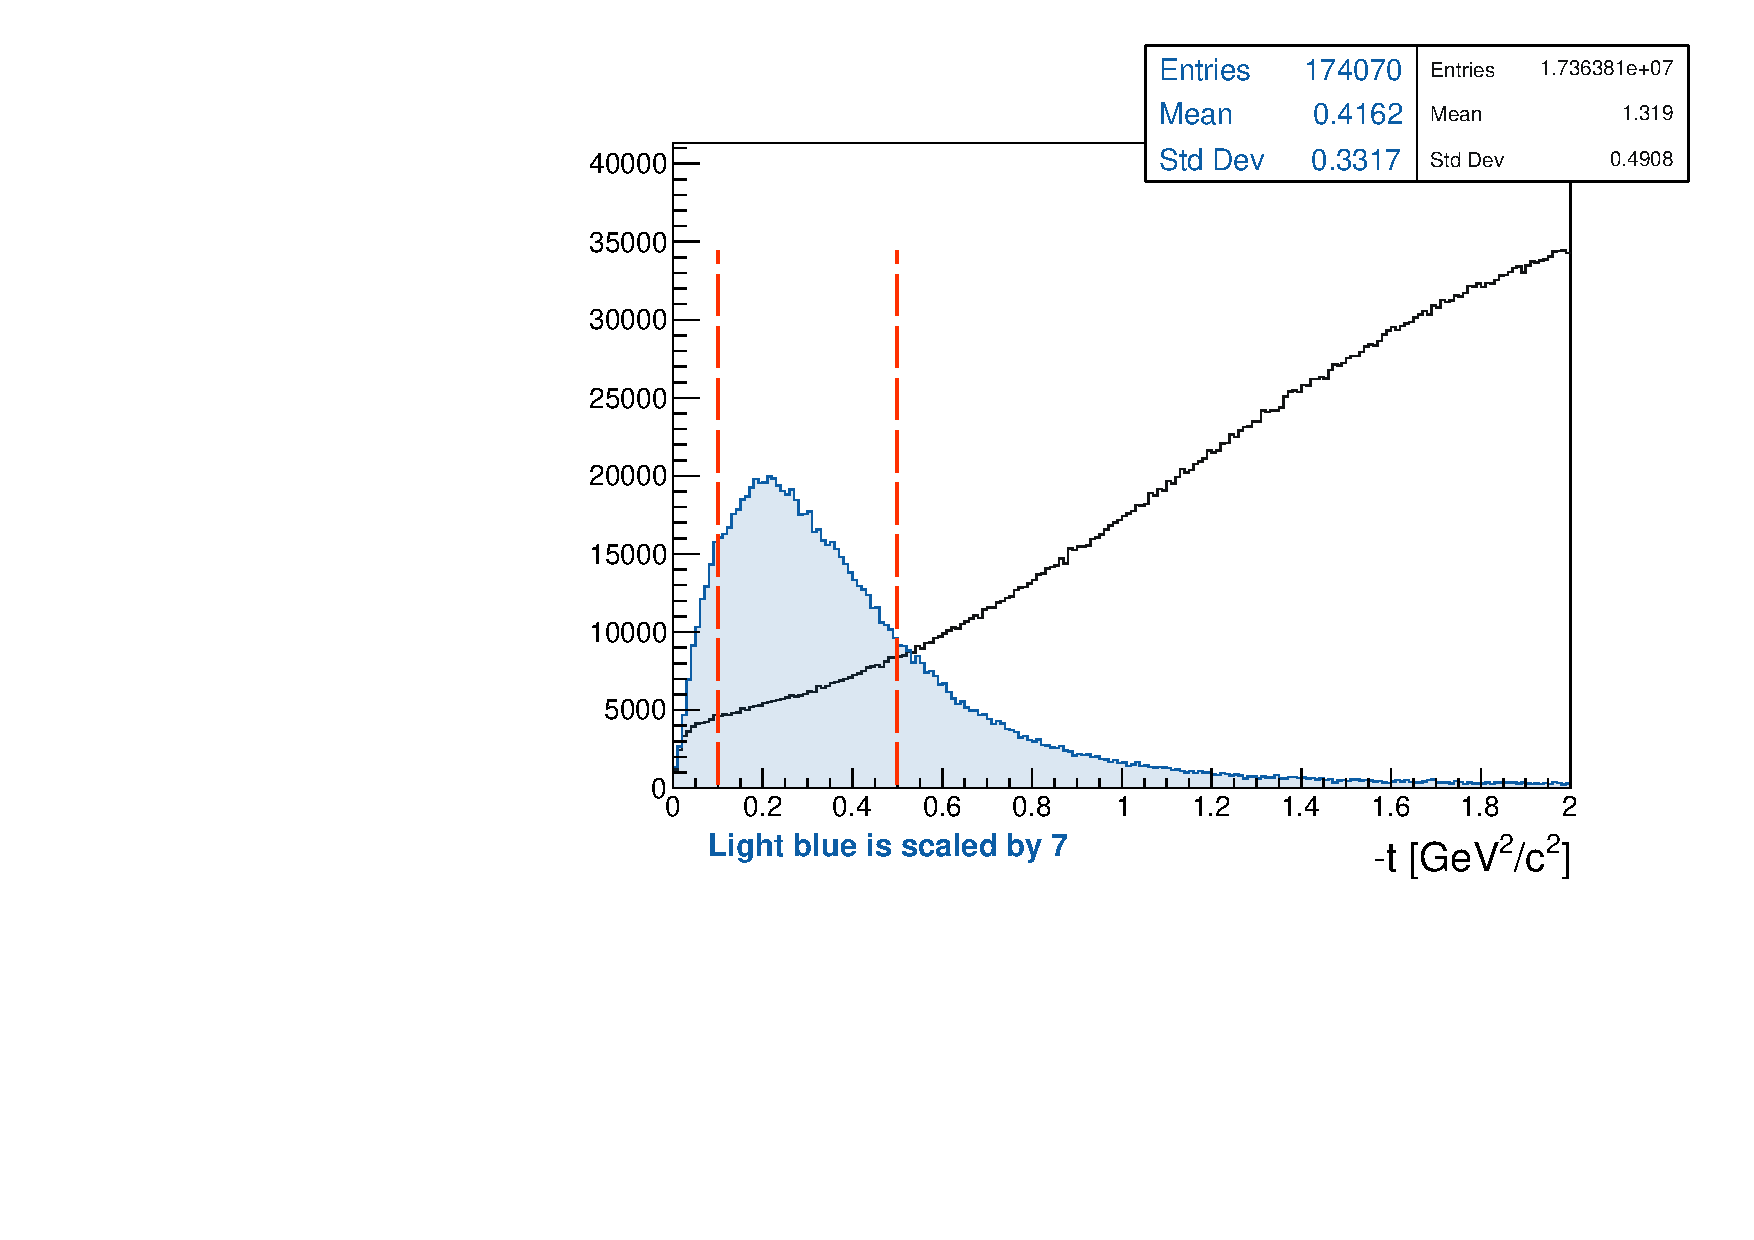
\includegraphics[width=280pt]{/work/clas12/ouillon/Analysis_RG-D/plots_Matt_Study/CxC/event_kinematics/pdf/t.pdf}
    \end{minipage}

    \begin{minipage}{.5\textwidth}
        \centering
        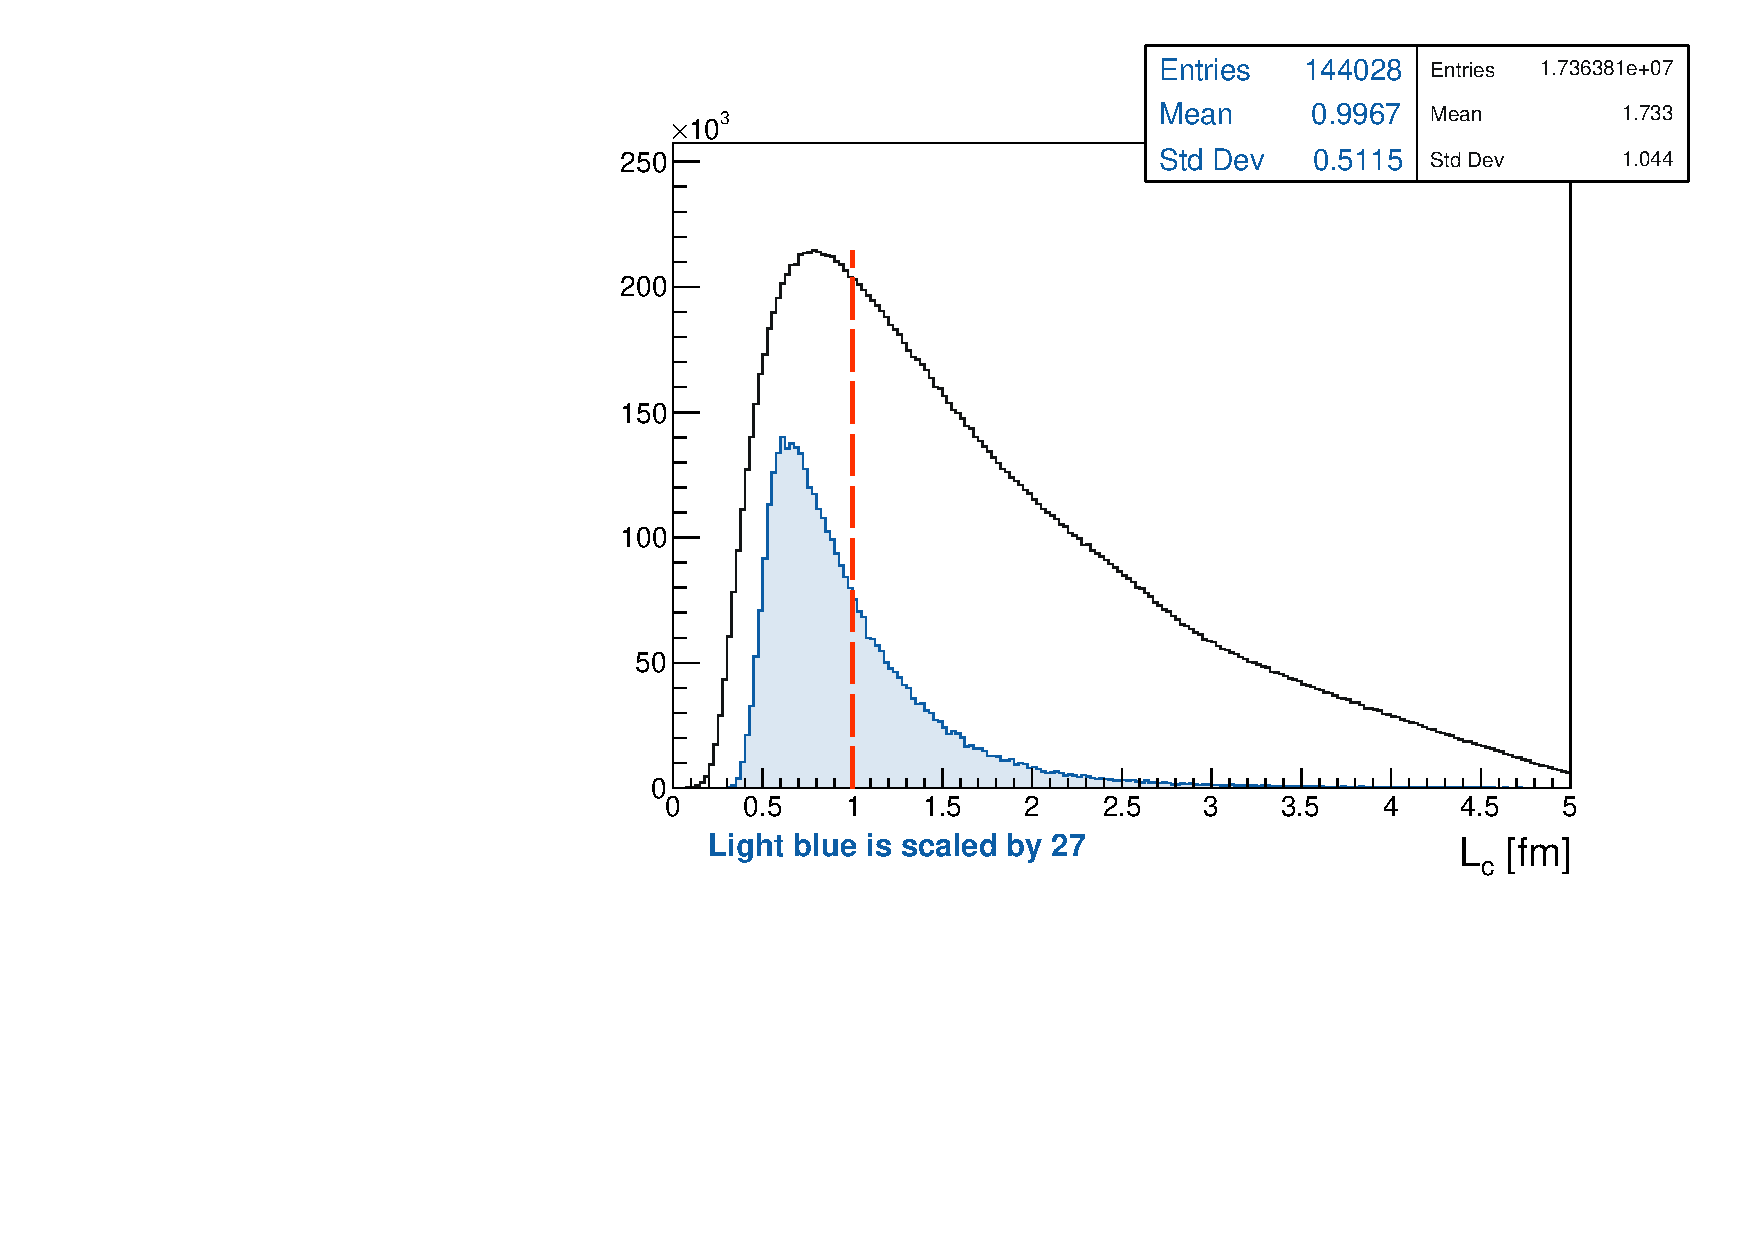
\includegraphics[width=280pt]{/work/clas12/ouillon/Analysis_RG-D/plots_Matt_Study/CxC/event_kinematics/pdf/lc.pdf}
    \end{minipage}
    \begin{minipage}{.5\textwidth}
        \centering
        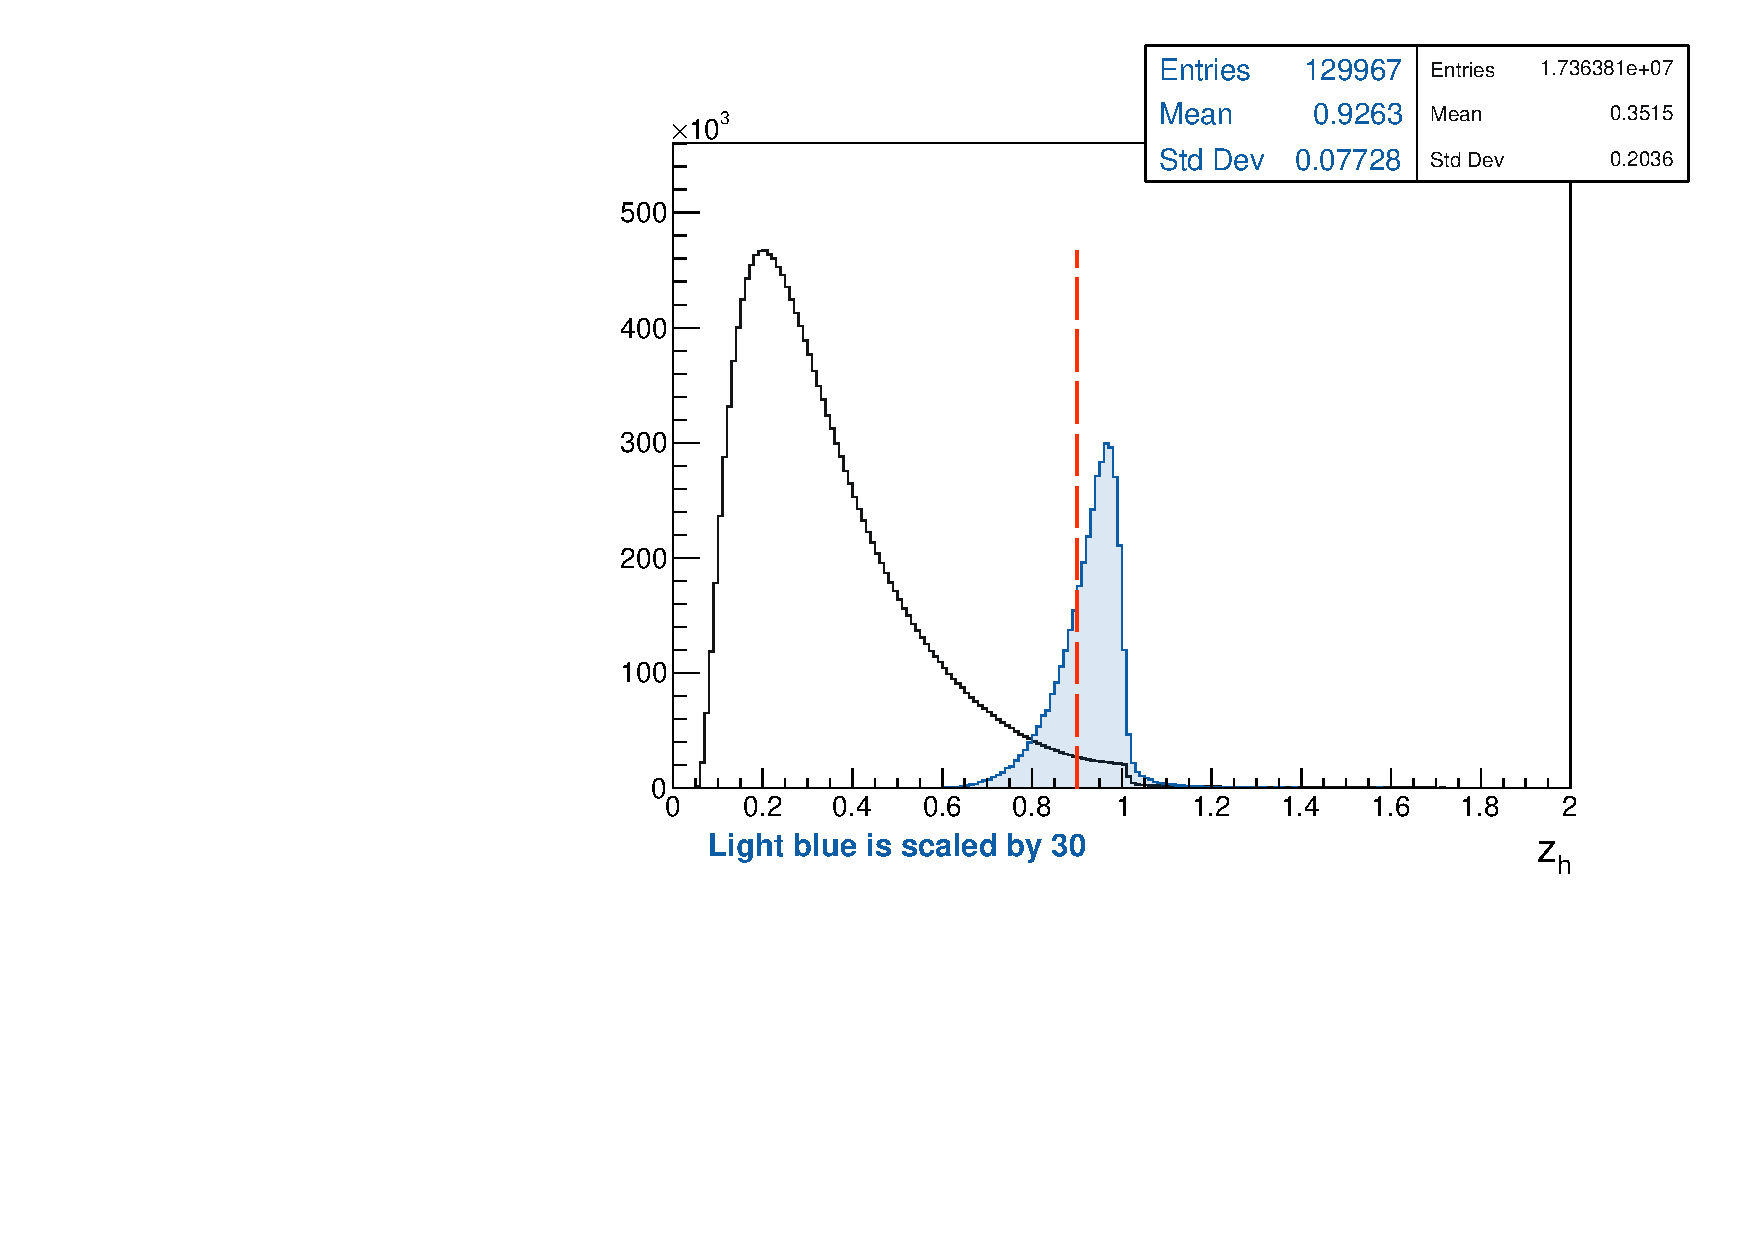
\includegraphics[width=280pt]{/work/clas12/ouillon/Analysis_RG-D/plots_Matt_Study/CxC/event_kinematics/pdf/zh.pdf}
    \end{minipage}

    \subsection{\(\rho^0\) invariant mass}
    \begin{minipage}{.5\textwidth}
        \centering
        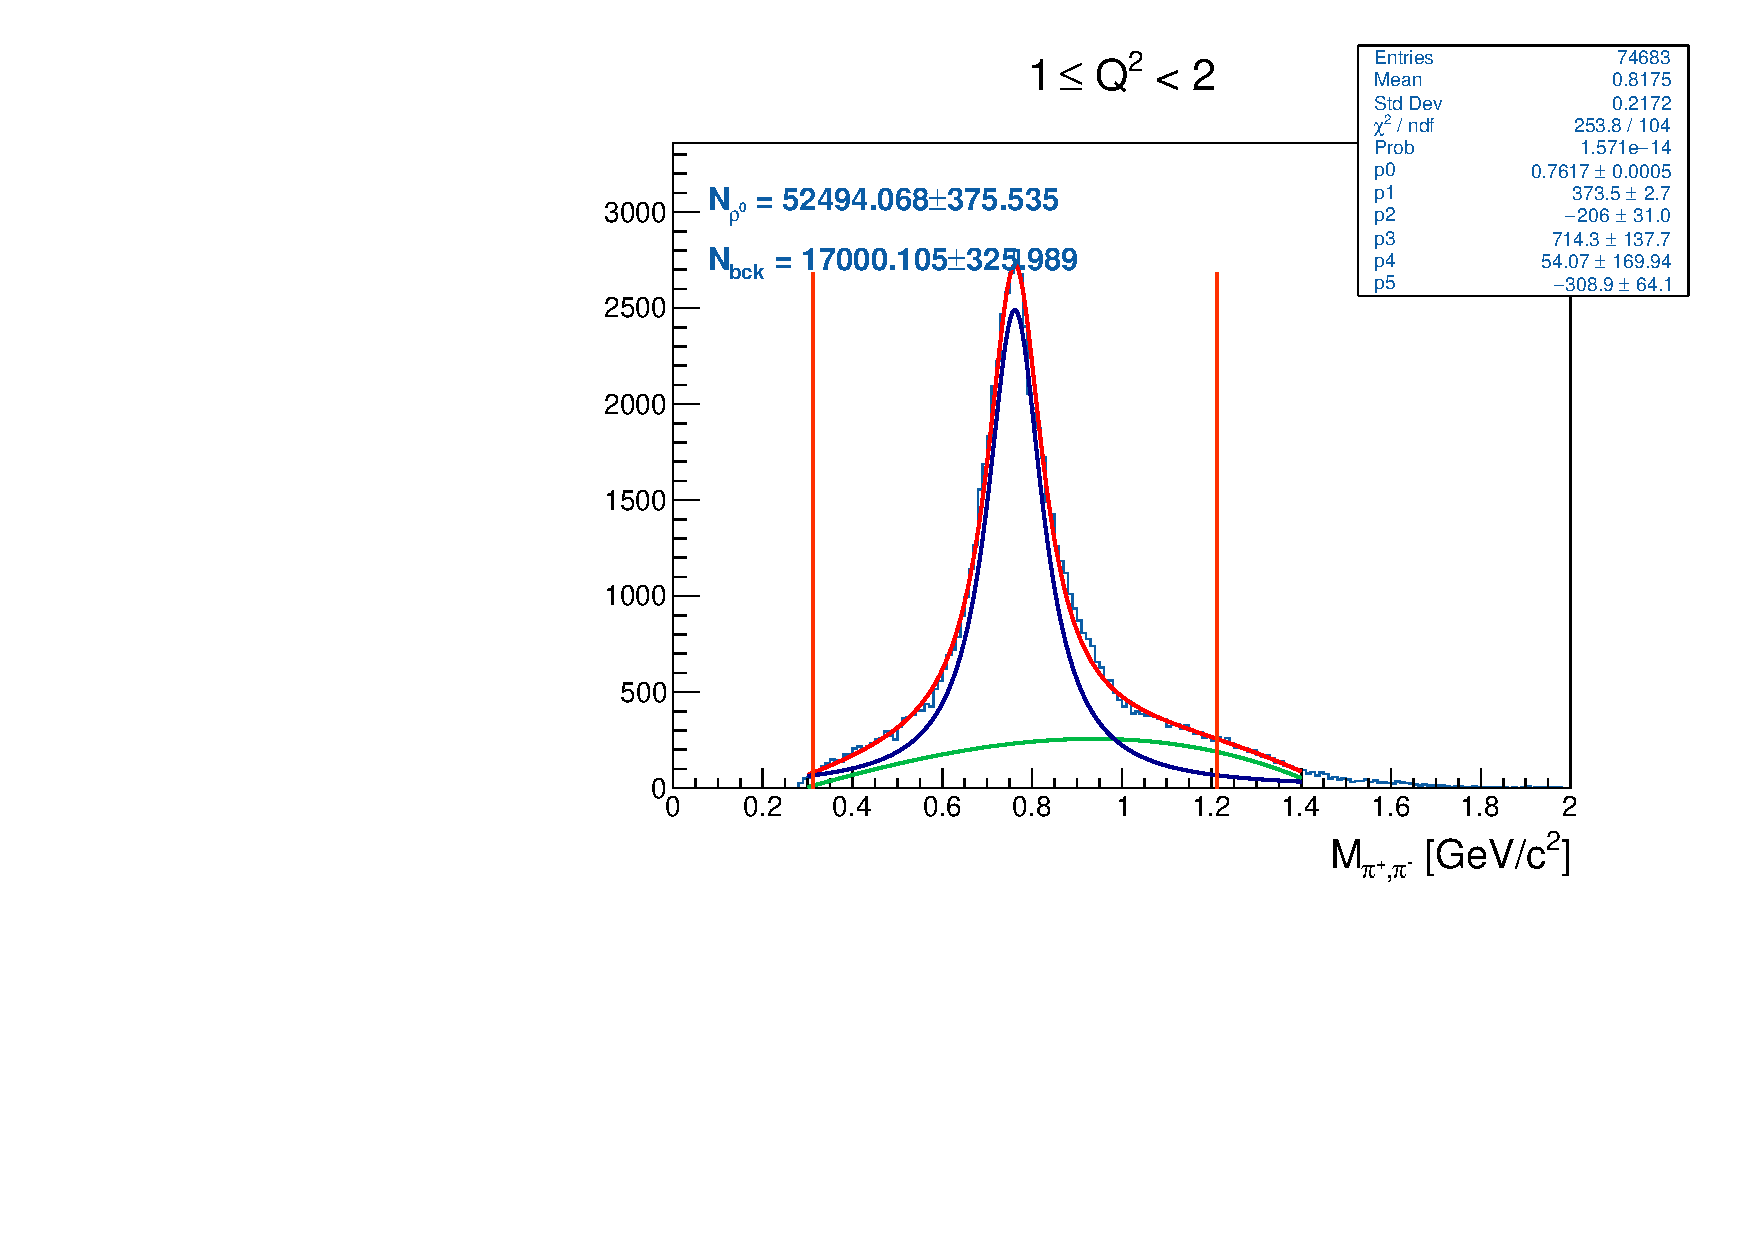
\includegraphics[width=280pt]{/work/clas12/ouillon/Analysis_RG-D/plots_Matt_Study/CxC/inv_mass_q2_bins/pdf/inv_Mass_Q12.pdf}
    \end{minipage}
    \begin{minipage}{.5\textwidth}
        \centering
        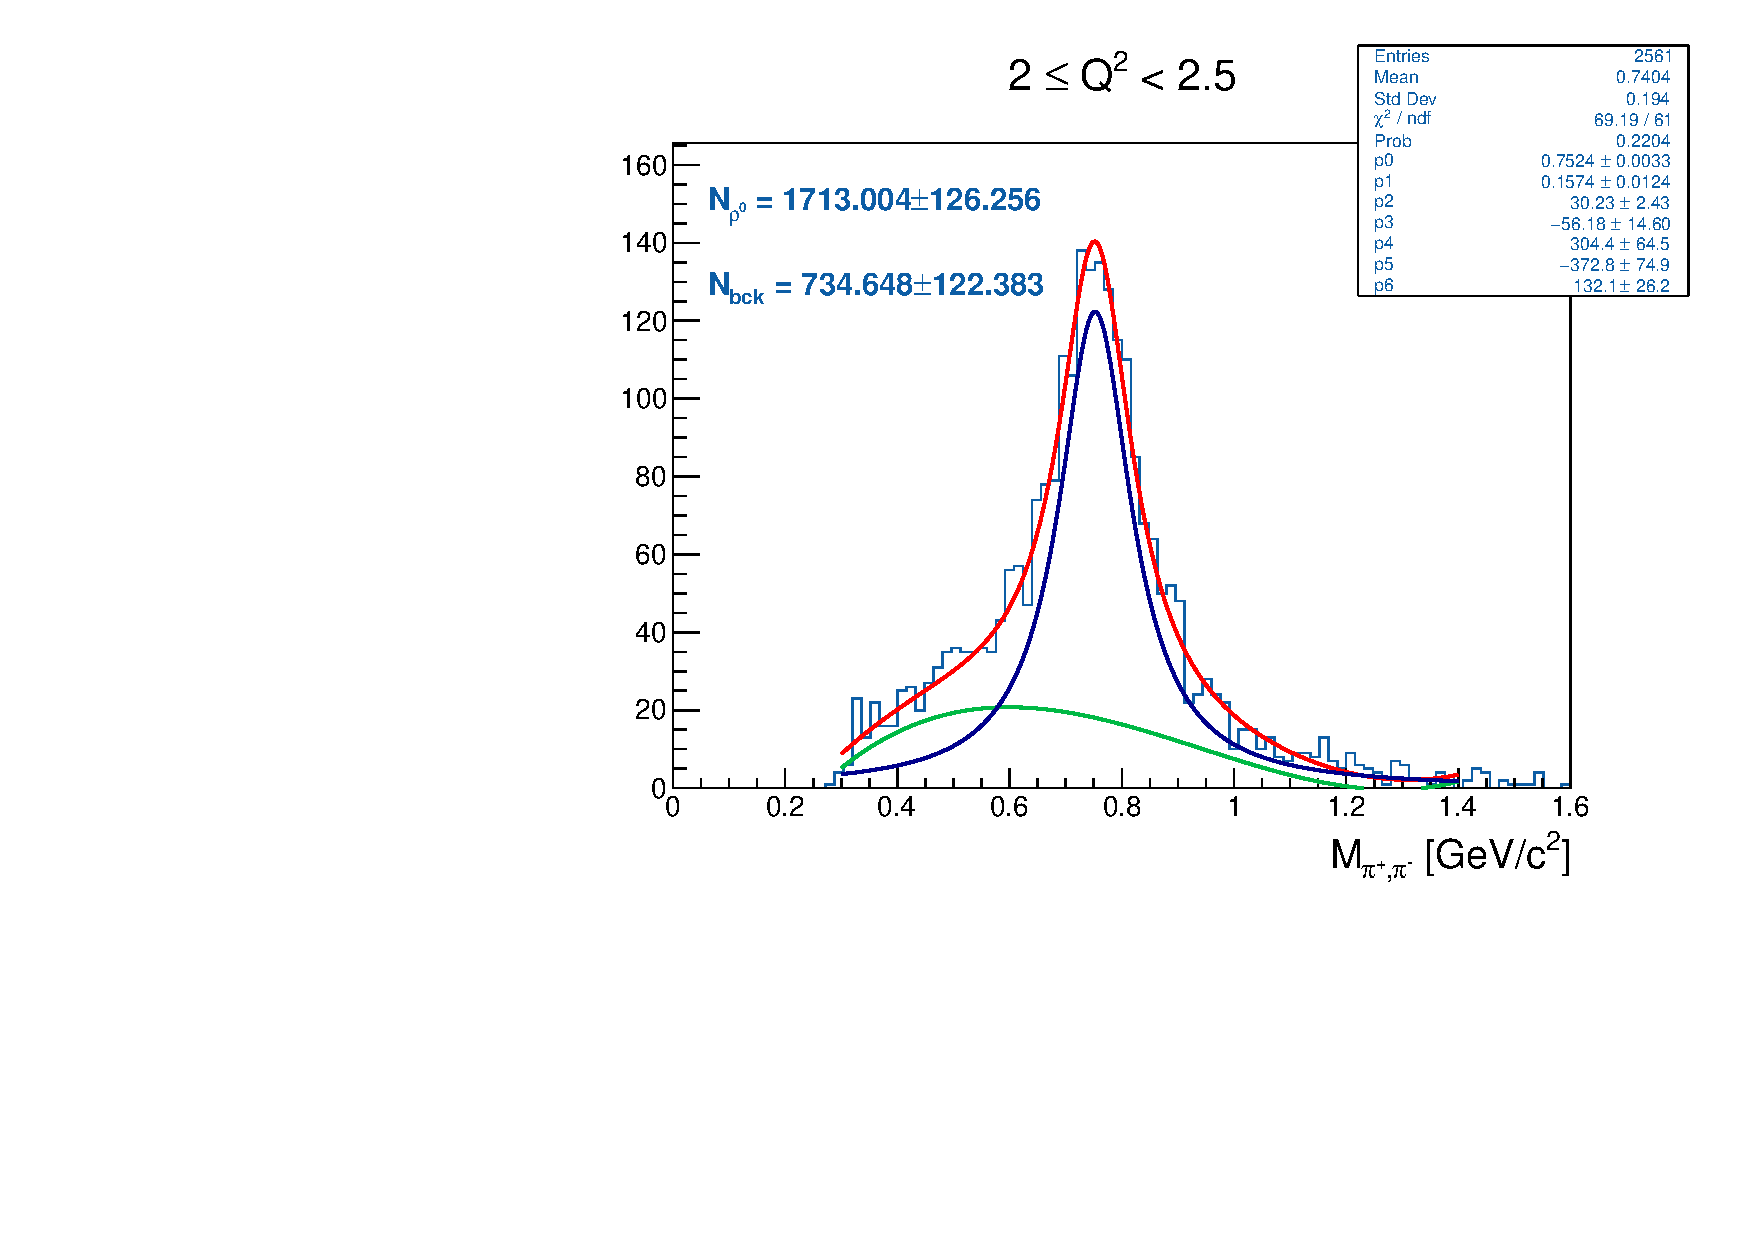
\includegraphics[width=280pt]{/work/clas12/ouillon/Analysis_RG-D/plots_Matt_Study/CxC/inv_mass_q2_bins/pdf/inv_Mass_Q225.pdf}
    \end{minipage}

    \begin{minipage}{.5\textwidth}
        \centering
        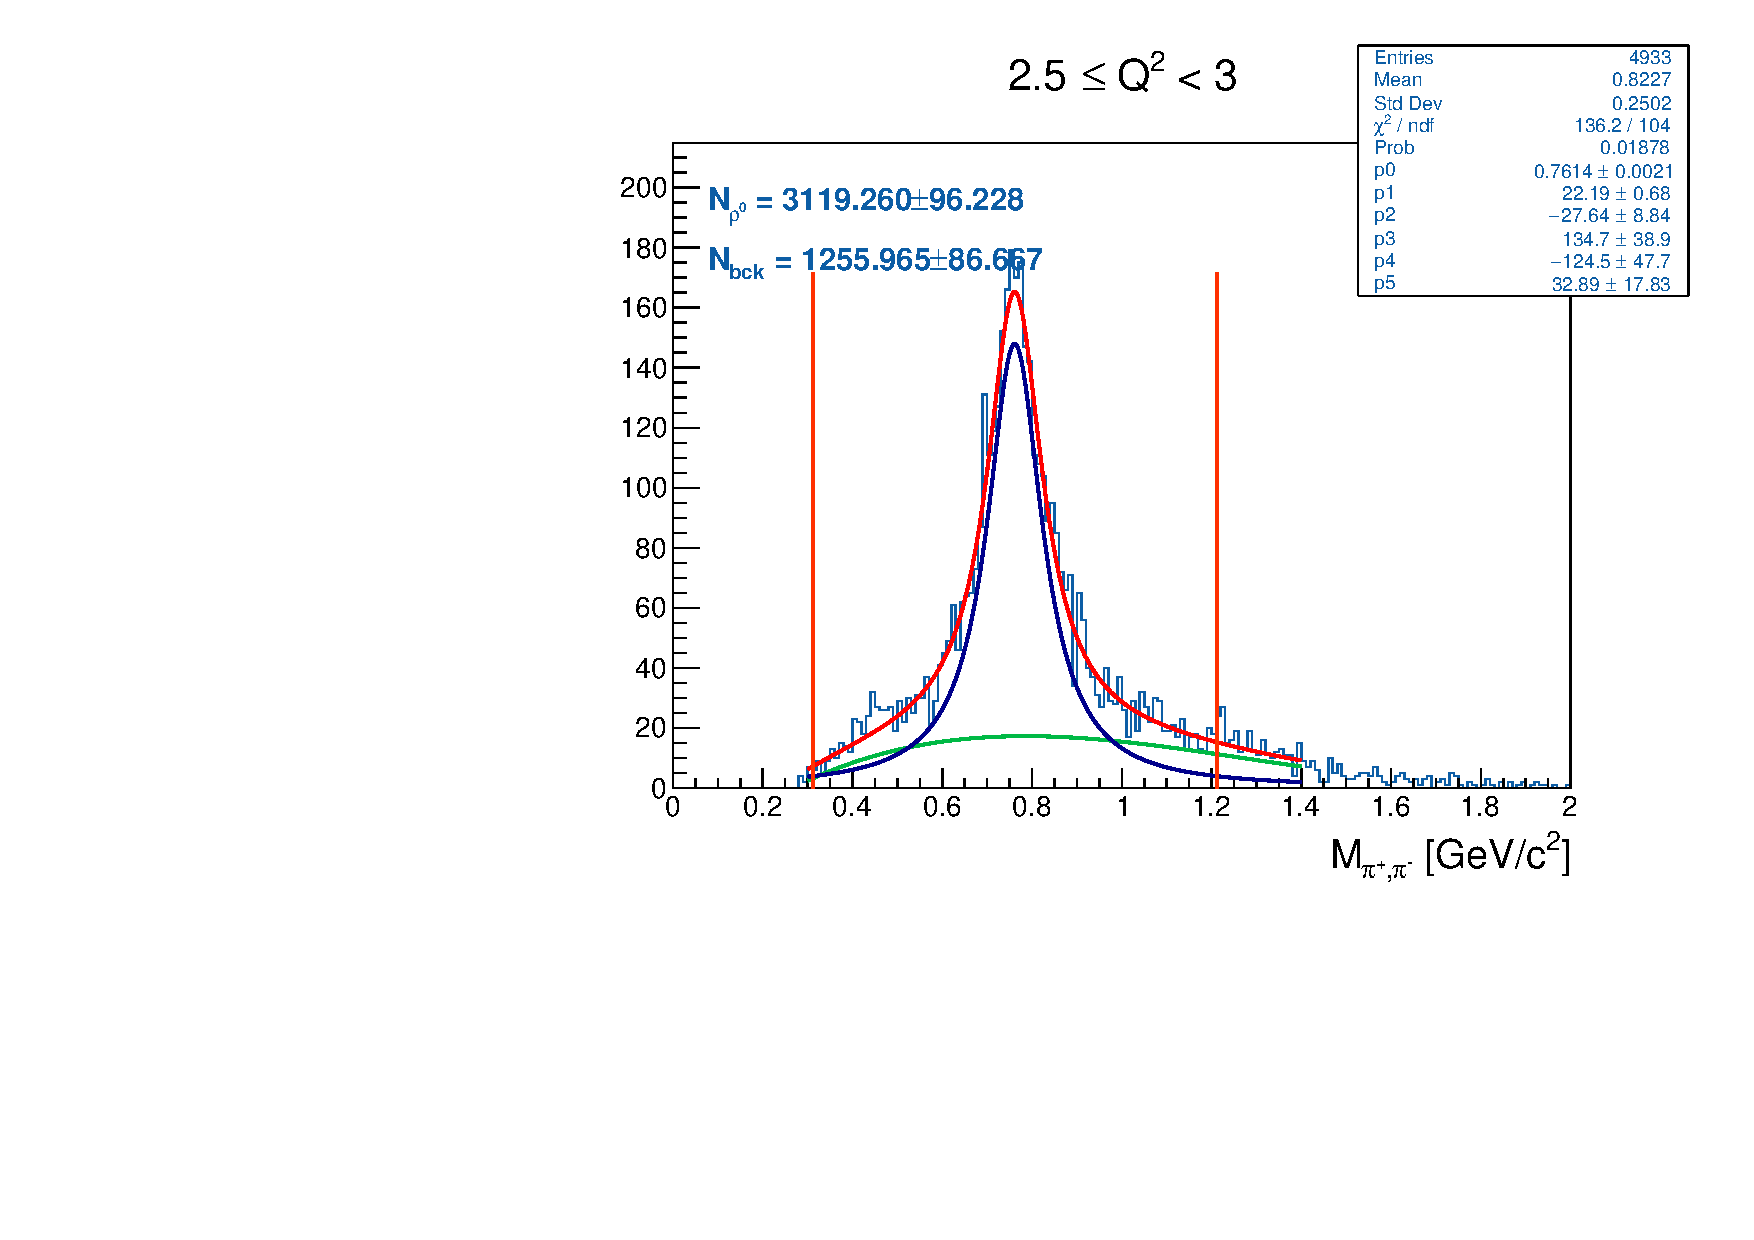
\includegraphics[width=280pt]{/work/clas12/ouillon/Analysis_RG-D/plots_Matt_Study/CxC/inv_mass_q2_bins/pdf/inv_Mass_Q253.pdf}
    \end{minipage}
    \begin{minipage}{.5\textwidth}
        \centering
        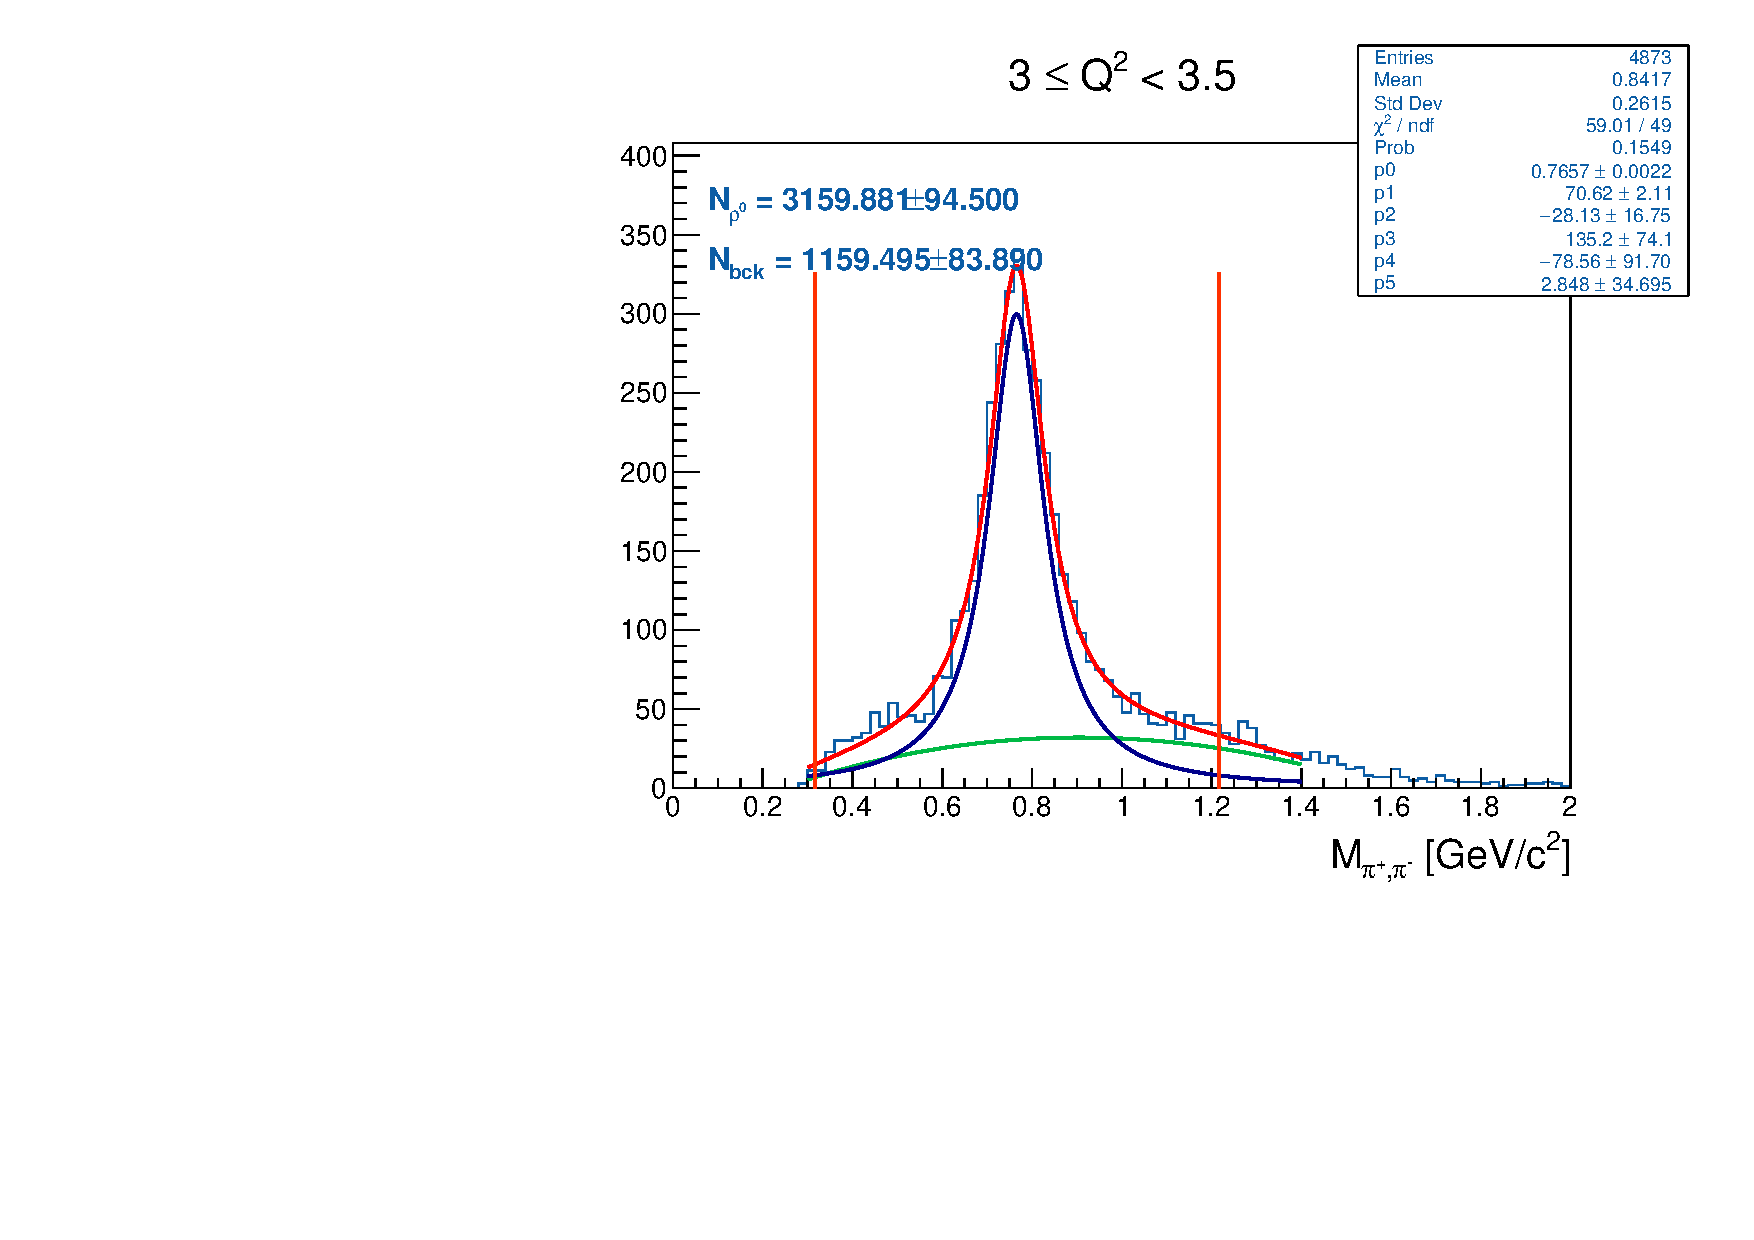
\includegraphics[width=280pt]{/work/clas12/ouillon/Analysis_RG-D/plots_Matt_Study/CxC/inv_mass_q2_bins/pdf/inv_Mass_Q335.pdf}
    \end{minipage}

    \begin{minipage}{.5\textwidth}
        \centering
        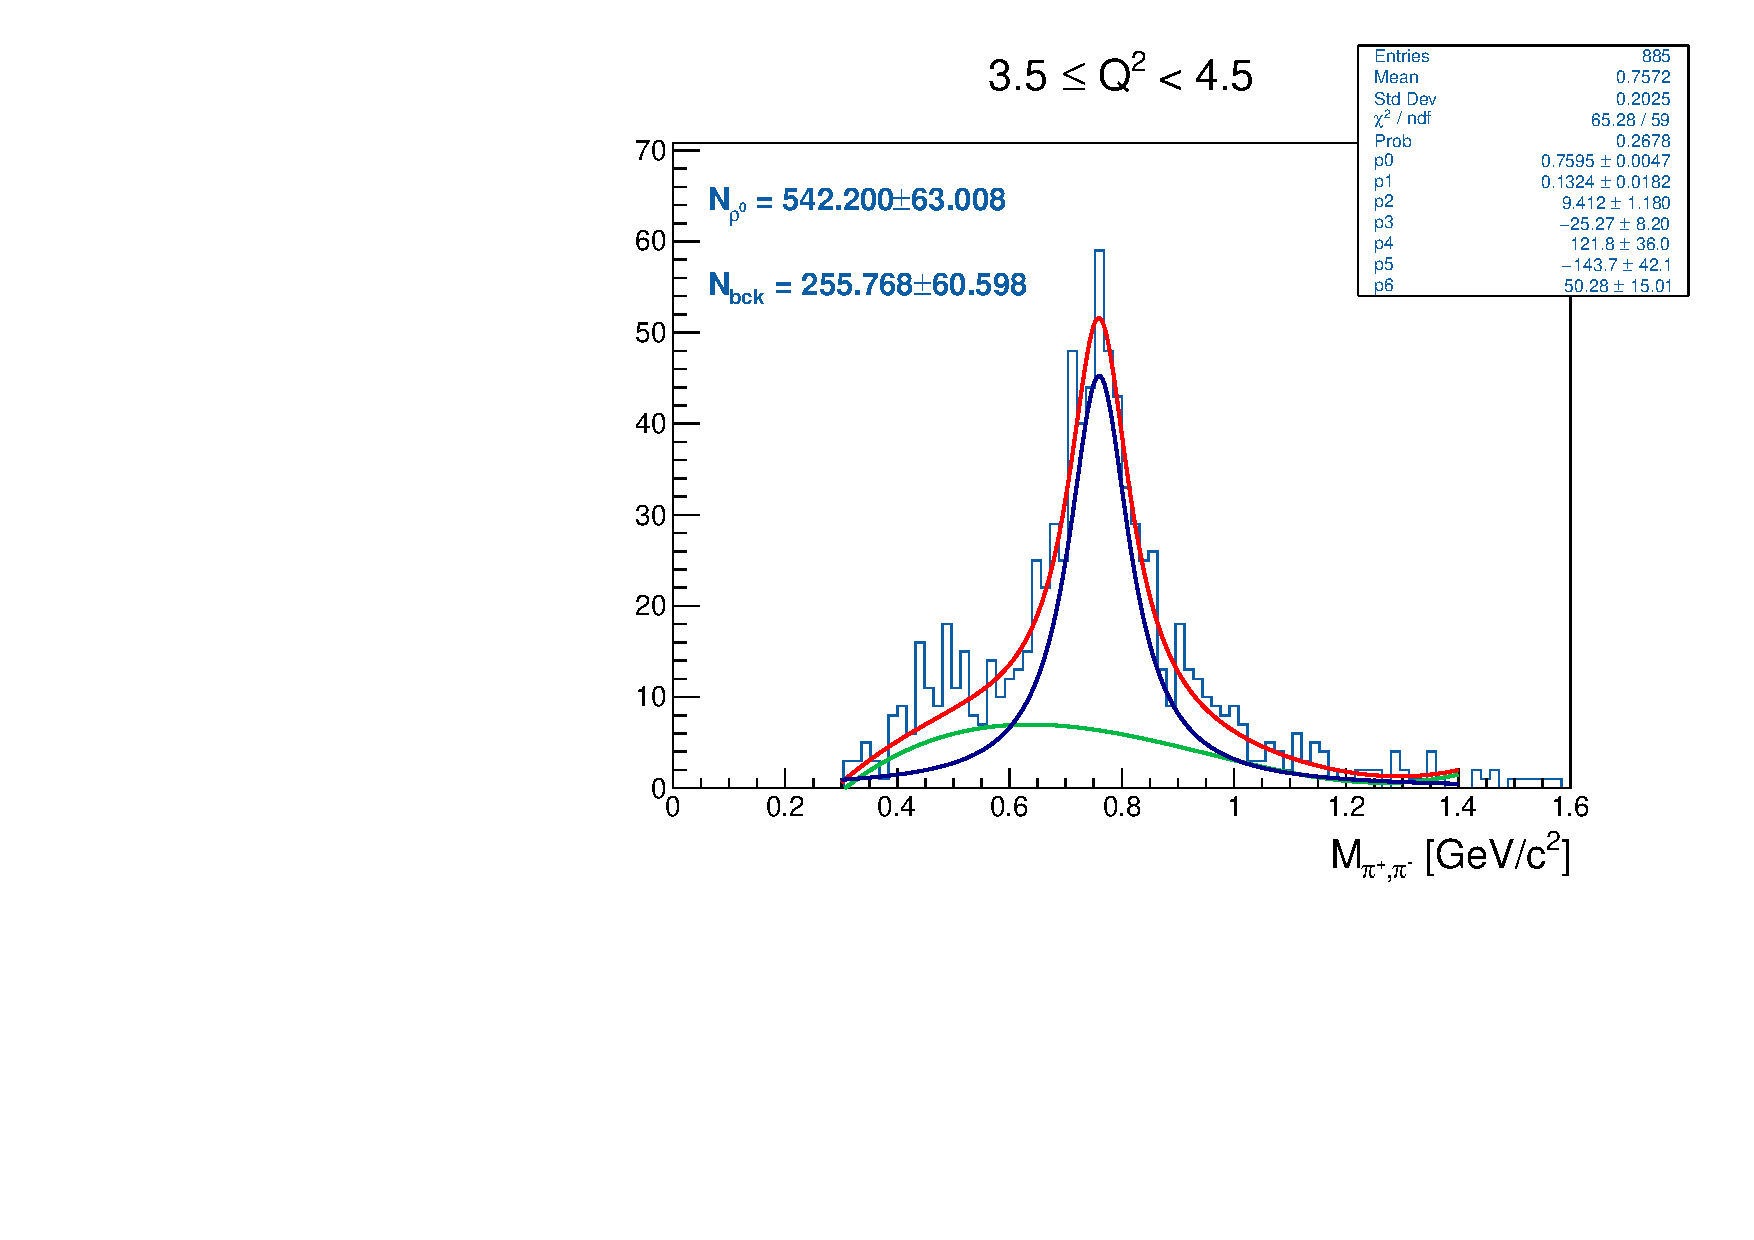
\includegraphics[width=280pt]{/work/clas12/ouillon/Analysis_RG-D/plots_Matt_Study/CxC/inv_mass_q2_bins/pdf/inv_Mass_Q3545.pdf}
    \end{minipage}
    \begin{minipage}{.5\textwidth}
        \centering
        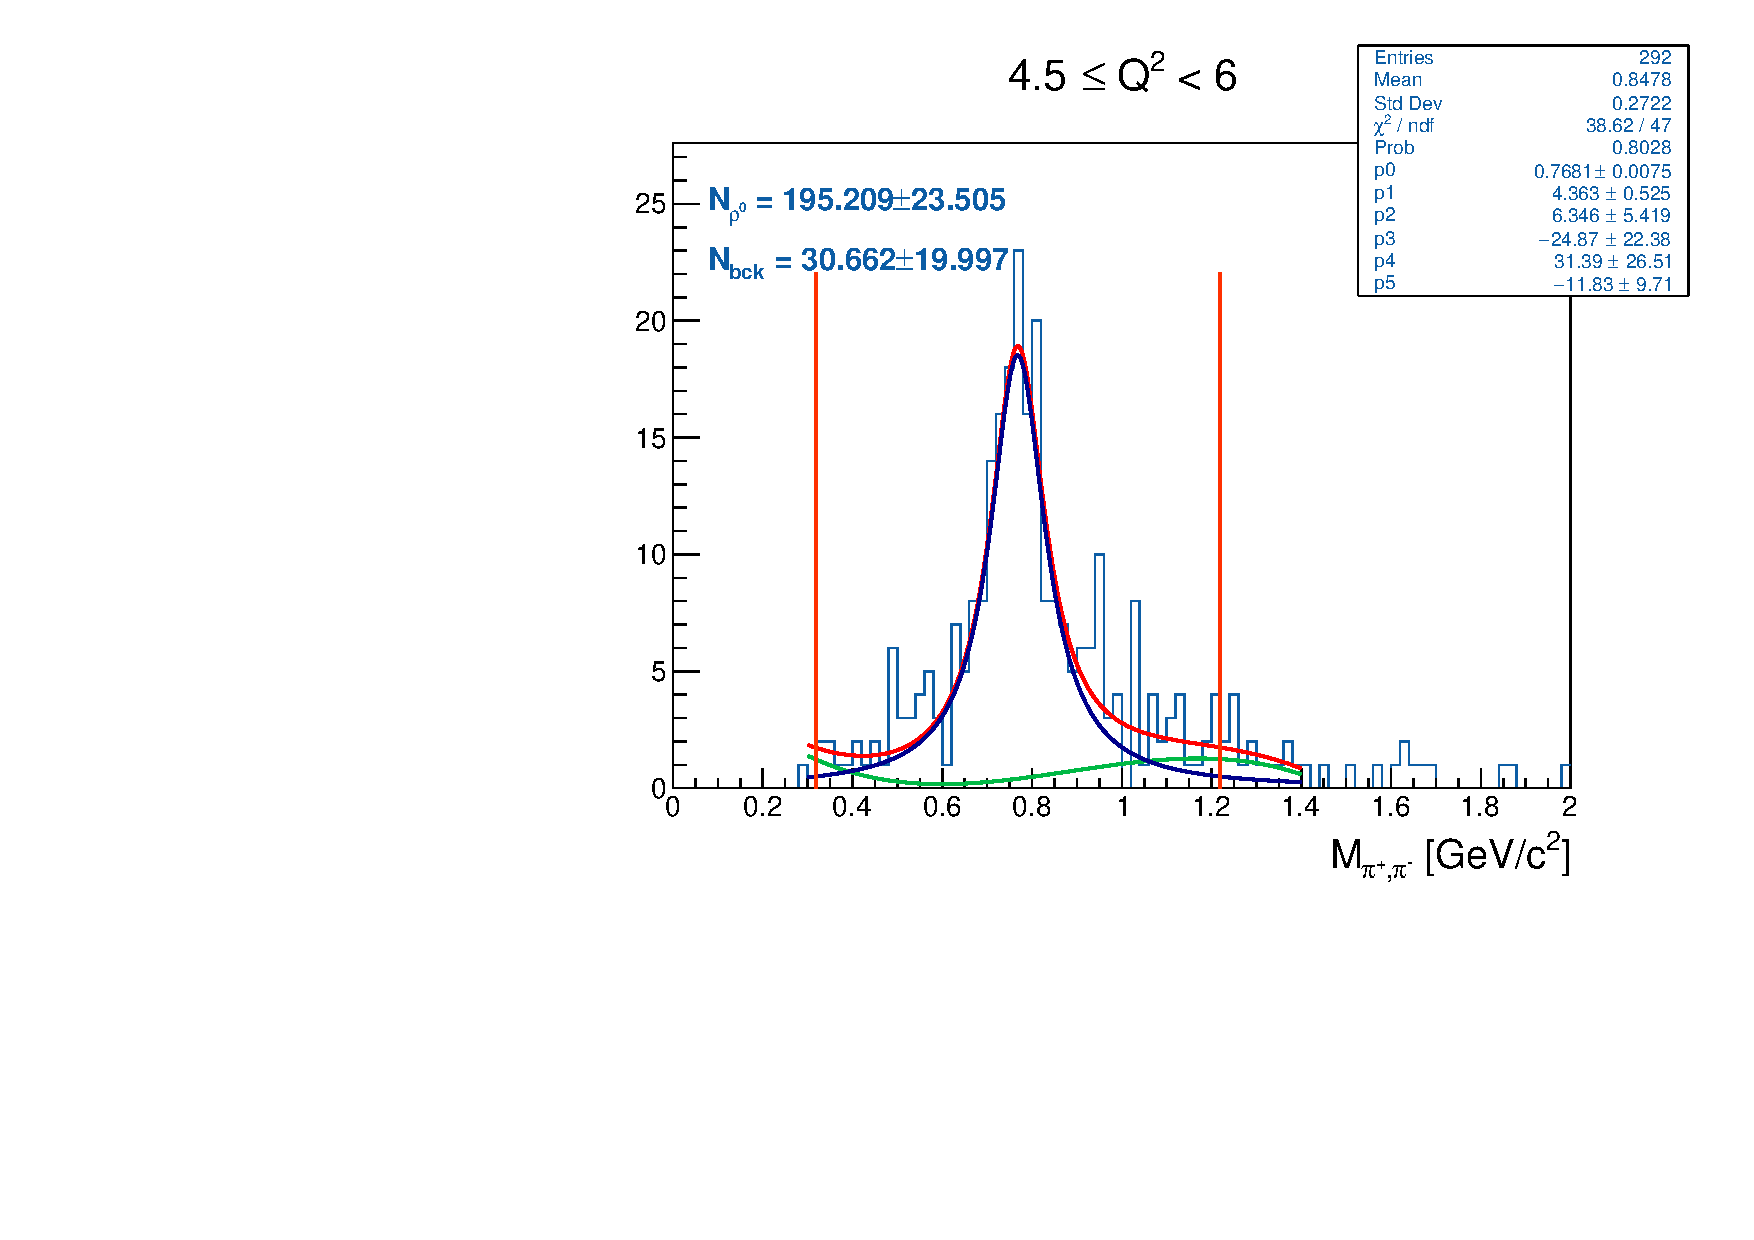
\includegraphics[width=280pt]{/work/clas12/ouillon/Analysis_RG-D/plots_Matt_Study/CxC/inv_mass_q2_bins/pdf/inv_Mass_Q456.pdf}
    \end{minipage}


    \subsection{LD2}
    LD2 runs : 018419, 018421, 018424, 018427, 018428, 018429, 018431, 018432, 018433, 018439, 018528, 018559, 018644, 018656, 018851, 018873, 019021, 019058
    
    path: \texttt{/cache/hallb/scratch/rg-d/production/Bspot/v5dstLD2/dst/recon/}
    \begin{itemize}
        \item Select the trigger electron: \texttt{REC::Particle::pid == 11} and \texttt{status<0}
        \item Apply cut on electron: \(-3 < \chi^2_{pid} < 3\) and \(-12 < v_z < 5\)
        \item Find all \(\pi^+\) in event: \texttt{REC::Particle::pid == 211}
        \item Apply cut on \(\pi^+\): \(-10 < \chi^2_{pid} < 10\) 
        \item Find all \(\pi^-\) in event: \texttt{REC::Particle::pid == -211}
        \item Apply cut on \(\pi^-\): \(-10 < \chi^2_{pid} < 10\) 
        \item Find all combination of \(\pi^+\) and \(\pi^-\)
        \item Cut to select reaction : 
        \begin{itemize}
            \item \(W = (p_i + \gamma^{\star})^2 > 2GeV\)
            \item \(z_h = \frac{E_{\rho^0}}{v}> 0.9\)
            \item \( 0.1 < -t < 0.5 GeV^2\)
            \item \(l_c \le 0.5 fm\)
        \end{itemize} 
    \end{itemize}

\end{document}